\documentclass[b5paper,opensource,sourcefont,parskip]{qyxf-book}
\usepackage{subcaption}
\usepackage{draftwatermark}
\usepackage{fontawesome5}
\SetWatermarkText{钱院学辅}
\SetWatermarkLightness{0.92}
\SetWatermarkScale{0.9}

% --------------------警告--------------------
% 由于副标题较长,因此私自在使用的qyxf-book.cls
% 文件中将副标题的字体尺寸由 \Huge 改为了 \huge,
% 请其他人编译时注意。
% --------------------------------------------

\title{大学物理题解(上)}
\subtitle{Key to University Physics: Part I}
\author{钱院学辅大物编写小组}
\typo{钱院学辅排版组}
\date{2019 年 6 月 9 日}
\version{v1.0}
\sourcepage{\url{https://github.com/qyxf/BookHub/}}


\newcommand{\di}[1]{\mathrm{d}#1}
\newcommand{\p}[2]{\frac{\partial #1}{\partial #2}}
\newcommand{\pp}[2]{\frac{\partial ^2 #1}{\partial #2 ^2}}
\newcommand{\dy}[2]{\frac{\di{#1}}{\di{#2}}}
\newcommand{\ddy}[2]{\frac{\mathrm{d} ^2 #1}{\mathrm{d} #2 ^2}}
\newcommand{\zbj}[4]
{
	\draw (0,0) node[below left] {$ O $};
	\draw [->] (#1,0) -- (#2,0) node[right] {$ x $};
	\draw [->] (0,#3) -- (0,#4) node[right] {$ y $};
}

\usepackage{siunitx}%输入角度
\usepackage{color}
\renewcommand{\thefootnote}{\color{red}\arabic{footnote}}%更改脚注格式

\begin{document}


\pagestyle{plain}
\chapter*{前言}
大学物理(University Physics)是本校理工科学生在大一、大二年级所要学习的一门自然科学
基础课程。这门课程课时较多、内容丰富,相关的练习题与考试题则尤显花样繁多,充分考验着每一个
学生对相关知识的掌握程度与应用能力。从掌握知识的角度来说,多做、精做大物习题是学好这门
课程的必经之路;从备考、应试的角度来说,若不熟练掌握各类大物习题的思路与解法,而仅依靠课内所
学到的基本知识点,则不可能在考试中取得令人满意的成绩。因此,熟练掌握本课程相关练习题的
解题技巧,是非常必要的。

目前,大多数大学物理的课堂均以一套统一印制的活页练习题作为课下作业。这套题目按章布置,
每章均有选择题、填空题、计算题三个部分,题量适中,覆盖了各章所有较为重要的知识点,并能
够使同学们充分地将课上所学知识用于实际问题的解决过程中。基于种种原因,这份题目的答案未见
公开;这能够保证大多数同学独立地完成作业,但不利于大家检查错误、在参考过程中发现自己的
问题。

为了解决这一问题,自2019年3月以来,钱院学辅组织了一些正在学习本课程的同学,编写了这份
大学物理题解(目前仅涵盖上半学期的相关内容)。该题解囊括了这一学期布置的所有作业之题解,
均有较详细的分析与求解过程可供参考。全书始终采用\LaTeX 整理,这使得本题解的排版效果得到
了充分的保证。我们希望,这份精心制作的题解,能够给正在学习与将要学习这门课程的同学提供
充分的帮助,使他们能够更好的掌握这项重要的基础课之内容。

本题解由\textbf{钱院学辅大物编写小组}完成,成员包括(按姓名拼音顺序):钱学森84班费立涵、
化生81班高旭帆、钱学森84班李浩天。其中,费立涵编写了第二、四、七章及第
一章计算题部分,李浩天编写了第三、五、八章,高旭帆编写了第六、九章及第一章的选择题与填空
题部分。钱院学辅学研部的越杰81班唐智亿、自动化钱71班吴思源与能动少C71班尤佳睿参加了稿件
的整理、校对、汇总与发布工作。在此,应向这些同学——特别是花费课余时间撰写题解的同学们表示
感谢。

“不积跬步,无以至千里。”一份可靠的题解,需要经过多次的改进才可望真正铸造出来。虽然这份题解的确可谓“精心制作”,但
笔误、错漏等在所难免,特别需要各位使用者帮助我们指正。如您在参考的过程中发现有任何错误
之处,欢迎您通过下面的方式联系我们,帮助我们改进这份题解:
\begin{itemize}
	\item \faGithub ~~ GitHub平台论坛(\textbf{推荐,但需要注册}):\url{https://github.com/qyxf/BookHub/issues}
	\item \faInternetExplorer ~~ 钱院学辅信息发布站:\url{https://qyxf.github.io}
	\item \faEnvelopeOpen ~~ 钱院学辅邮箱:\texttt{qianxiaofu.mail@qq.com}
	\item \faQq ~~ 钱院学辅官方答疑墙:~~\textbf{钱小辅}~~206713407
\end{itemize}

作为钱院学辅出品的第一份“重量级”作品,希望它能够带给每一位同学最好的体验!

\begin{flushright}
钱院学辅大物编写小组\\
2019 年 6 月 9 日
\end{flushright}
\vspace{1.0cm}
\begin{figure}[!h]
	\centering
	\begin{minipage}[c]{0.5\textwidth}
		\centering
		
\includegraphics[scale=0.5]{qrcode2.png}
	\end{minipage}%
	\begin{minipage}[c]{0.5\textwidth}
		\centering
		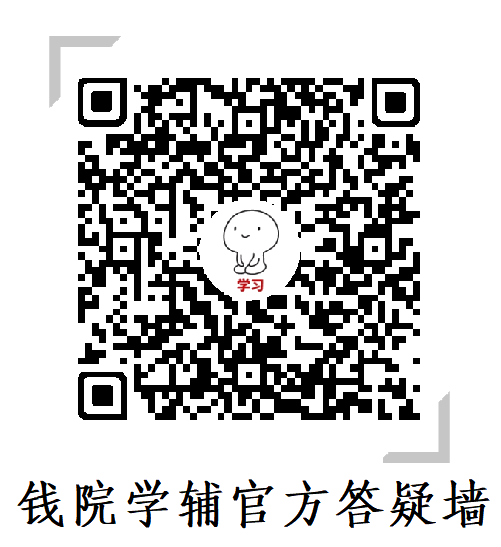
\includegraphics[scale=0.5]{qxf.png}
	\end{minipage}
\end{figure}


\cleardoublepage

\tableofcontents

\setlength{\parindent}{0pt}
\chapter{质点运动学及牛顿运动定律}
\section{选择题}
\exercise{1}A

\solve 如图1.1,对$M$,在$x$方向上:
\begin{figure}[htbp]
	\centering
	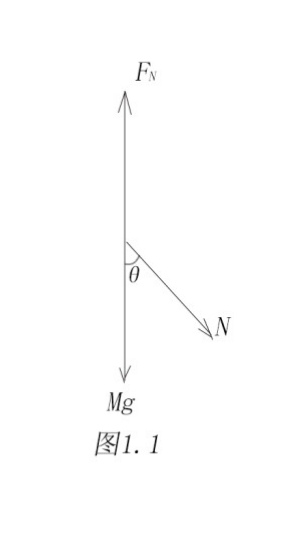
\includegraphics[width=10em,height=15em]{Chp1_illus1.png}
	\quad
	\centering
	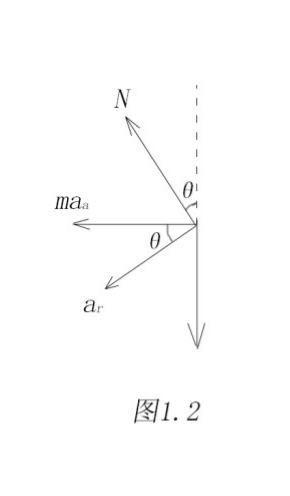
\includegraphics[width=10em,height=15em]{Chp1_illus2.png}
\end{figure}
\begin{equation}
N\sin\theta=Ma_e\text{(M对地)}
\end{equation}
如图1.2,对$m$,以$M$为参考系,$m$受一惯性力,合加速度沿二者接触面。沿$x,y$方向分解:
\begin{gather}
mg-N\cos\theta=ma_r\sin\theta\\
ma_e+N\sin\theta=ma_r\cos\theta
\end{gather}
将(1)代入(2),由(2)(3)联立解得:
\[a_r=\dfrac{(M+m)g\sin\theta}{M+m{\sin\theta}^2}\]


\exercise{2}B

\solve 如图1.3,$u=v\cos\theta$,v不变而$\theta$增大,需要u减小。

\begin{figure}[htbp]
	\centering
	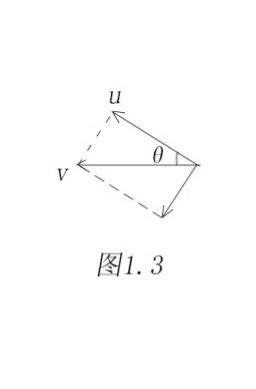
\includegraphics[width=6.5em,height=10em]{Chp1_illus3.png}
	%\caption{}
	\label{fig:Chp1_illus2}
\end{figure}


\exercise{3}A

\solve 匀速圆周运动的速度、加速度(受力)均是大小不变、方向时刻变化。
注意一个矢量为常量包括大小和方向两个方面。否则就是变化的量。

\exercise{4}B

\solve 以前面的货车为参考系,货车静止,火车速率为$v_1-v_2$,加速度为$a$(反向),那么火车最多前进$s=\dfrac{{(v_1-v_2)}^2}{2a}$。要求$d>s$,故选B。或采用地面参考系的追逐问题法,计算从$v_1\text{减速到}v_2$两车走过的距离之差为
\[
s=\dfrac{{v_1}^2-{v_2}^2}{2a}-v_2\cdot \dfrac{v_1-v_2}{a}=\dfrac{{(v_1-v_2)}^2}{2a}.
\]

\exercise{5}C

\solve 两次求导得:$a=30t$,不等于常数而大于零。

\exercise{6}B

\solve 求导得:$v=8t-6t^2,a=8-12t$

令$y=0\Rightarrow t=0\text{(舍去)或}2$s,代入得结果。

\exercise{7}B

\solve 物体做匀加速直线运动。
\begin{gather*}
s=\dfrac{b}{\cos\alpha},a=g\sin\alpha\\
t=\sqrt{\dfrac{2s}{a}}=\sqrt{\dfrac{4b}{g\sin(2\alpha)}}
\end{gather*}
当$t$最小时,$\sin(2\alpha)$最大,$\alpha=45^\circ$。

\exercise{8}B

\solve 类比从静止出发的匀加速直线运动。$\dfrac{1}{2}\beta t^2=2\pi$

\exercise{9}B

\solve 曲线的定义:“动点运动方向连续变化的轨迹\footnote{来源:汉典网http://www.zdic.net/c/2/111/299079.htm}”。A,C的反例:匀速圆周运动。做曲线运动的物体一定有加速度。

\exercise{10}D

\solve 反例:平抛运动。

\section{填空题}
\exercise{11}$0$\qquad$2g$

\solve 设A、B质量为m。抽走C之前,弹簧中的弹力大小为mg。撤去C时,弹簧长度未突变,弹力不变,A受合力为0;支持力则消失。

故$a_A=0$,$a_B=\dfrac{mg+mg}{m}=2g$,竖直向下。

\exercise{12}$\dfrac{25}{12}\pi$ rad/$\textrm{s}^2$ \qquad$\dfrac{24}{5} \textrm{s}$

\solve 简单公式应用。
\begin{gather*}
\text{}\theta=60\times2\pi=120\pi\\
\beta=\dfrac{\omega_2^2-\omega_1^2}{2\theta}=\dfrac{25}{12}\pi\ rad/s^2\\
\Delta t=\dfrac{\omega_2-\omega_1}{\beta}=\dfrac{24}{5}s
\end{gather*}

\exercise{13}$m(\sin\theta-\omega^2l\sin\theta\cos\theta)$

\begin{figure}[!htbp]
	\centering
	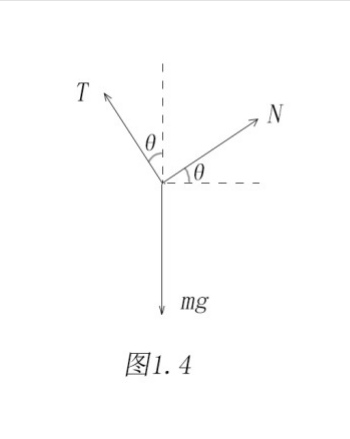
\includegraphics[width=15em, height=15em]{Chp1_illus4.png}
	%\caption{}
	\label{fig:c1}
\end{figure}

\solve 如图1.4,在$x$,$y$方向上分解受力,得:

\[\begin{cases}
T\sin\theta-N\cos\theta=m\omega^2l\sin\theta\\
T\cos\theta+N\sin\theta=mg
\end{cases}
\]
联立可解得$T$、$N$的大小。

\exercise{14}\ $2\sqrt{\dfrac{r}{g}}$ \qquad $2\sqrt{\dfrac{r}{g}}$

\solve 
设弦与PC的夹角为$\theta$,则有:
\begin{gather*}
s=2r\cos\theta,a=g\cos\theta\\
t=\sqrt{\dfrac{2s}{a}}=2\sqrt{\dfrac{r}{g}}
\end{gather*}
结果与$\theta$无关。


\exercise{15}$4\sqrt{5}\textrm{m/s}$ \qquad $16\textrm{m/s}^2$

\solve 抛物线的切线方向即为质点的速度方向,且$x=v_xt$。
\[
\dfrac{v_y}{v_x}=\dy{y}{x}=x\Rightarrow v_y=4x=16t
\]
$x=2$m时,$t=0.5$s,则:
\begin{gather*}
v_y=8\textrm{m/s}\\
v=\sqrt{{v_x}^2+{v_y}^2}=4\sqrt{5}\mathrm{m/s}
\end{gather*}
$v_x$不变,故:
\[
a=a_y=\dy{v_y}{t}=16\textrm{m/s}^2
\]

\exercise{16} 长度、质量、时间

\solve 见课本。

\exercise{17} 3\quad 3\quad 6

\solve $x$分别对$t$求一阶、两阶导,即是$v$、$a$,由图像即可判断其正负号。

\exercise{18} $y={(x+5)}^3$

\solve 由题,$x=2t-5\Rightarrow 2t=x+5$。

代入$y=8t^3={(2t)}^3$,消去t即可。

\exercise{19}$\dfrac{1}{2}g$\qquad 竖直向下

\solve 初始时受力平衡,两根弹簧上力均为$\dfrac{1}{2}mg$;一根断掉后,向上的力减半,则小球受的合力是$\dfrac{1}{2}mg$,竖直向下。

\exercise{20}$9$m/s

\solve 
\begin{align*}
\text{(SI)} x=3t+6t^2-2t^3&\xrightarrow{\text{求导}}v=3+12t-6t^2\\
&\xrightarrow{\text{求导}}a=12-12t
\end{align*}
令$a=0$,解得
\[
t=1\xrightarrow{\text{代入得}} v(1)=9\mathrm{m/s}
\]

\section{计算题}
\exercise{21}

\solve 
由图知:
\begin{gather*}
\tan\alpha=\dfrac{|\vec{a}_n|}{|\vec{a}_\tau|}=\dfrac{\frac{v^2}{R}}{\dy{v}{t}}\\
\frac{\di{v}}{v^2}=\frac{\di{t}}{R\tan\alpha}
\end{gather*}
积分得:
\[
-\frac{1}{v}=\frac{1}{R\tan\alpha}t+C
\]
代入$t=0,v=v_0$:
\[
C=-\dfrac{1}{v_0}\Rightarrow -\frac{1}{v}=\frac{t}{R\tan\alpha}-\dfrac{1}{v_0}
\]
所以:
\[
v=\frac{v_0R\tan\alpha}{R\tan\alpha-v_0t}
\]

\exercise{22}

\solve 
\begin{gather*}
\vec{v}=\dy{s}{t}\vec{\tau}=(c+2dt)\vec{\tau}\\  
\vec{a}_n=\frac{v^2}{R}\vec{n}=\frac{(c+2dt)^2}{R}\vec{n}\\
\vec{a}_\tau=\dy{v}{t}\vec{\tau}=2d\vec{\tau}
\end{gather*}
令$|\vec{a}_n|=|\vec{a}_\tau|$,则
\begin{gather*}
\frac{(c+2dt)^2}{R}=2d\\
t=t_1=\frac{\sqrt{2dR}-c}{2d}\left(t_2=\frac{-\sqrt{2dR}-c}{2d}<0\text{,舍去}\right)
\end{gather*}
$\therefore$要使$t\geqslant0$,条件为$\sqrt{2dR}-c\geqslant0$,即$2dR\geqslant c^2$。


\exercise{23}

\solve 根据已知条件有$-kx=a=\dy{v}{t}=\dy{v}{x}\cdot \dy{x}{t}=\dy{v}{x}\cdot v$,此即关于$x$与$v$的微分方程
\[-kx=\dy{v}{x}\cdot v\]
分离变量,积分得
\[-\dfrac{1}{2}kx^2=\dfrac{1}{2}v^2+C_1\]
令$C=2C_1$,则有$-kx^2=v^2+C$,进一步代入$x=x_0,v=v_0$得$C=-(kx_0^2+v_0^2)$。经过整理可得
\[v=\pm\sqrt{kx_0^2+v_0^2-kx^2}.\]


\exercise{24}

\solve (1) 易得$v=10\left(1-\dfrac{t}{5}\right)=-2t+10$,此即
\[
\dy{x}{t}=-2t+10
\]
积分得$x=-t^2+10t+c$,代入$t=0,x=0$可求得$c=0$。故有
\[x=-t^2+10t\]
代入$t=10s$得$x(10)=0$,即坐标为0。\\
(2) 令$x=10$m,则有$t^2-10t+10=0$,解得
\[t=5\pm\sqrt{15}\text{ s}\]
同理,令$x=-10$m,有$t^2-10t+10=0$,解得
\[t=5+\sqrt{35}(5-\sqrt{35}<0,\text{舍去})\]
综上可知,时刻为$5-\sqrt{15}$\ s,$5+\sqrt{15}$\ s或$5+\sqrt{35}$\ s。\\
(3) 令$v=0$,有$t=5$s,故可见对t\in[0,5],有$s=x=-t^2+10t$;而对$t\in[5,+\infty)$,有
\[s=s(5)+[s(5)-x]=25+[25-(-t^2+10t)]=t^2-10t+50\]
综上得$s=
\begin{cases}
-t^2+10t,&t\in[0,5)\\
t^2-10t+50,&t\in[5,+\infty)
\end{cases}$

\chapter{功和能}
\section{选择题}

\exercise{1}C

\solve 质点沿力方向位移为零,故$A=0$.

\exercise{2}B

\solve 可见$B$离开$A$时为弹簧恢复原长的时刻(该时刻之后,$A$受到弹簧拉力,加速度为负,$v_A<v_B$.),
此时$v_A=v_B$.由动能定理易得
\[\frac{1}{2}mv_A^2+\frac{1}{2}mv_B^2-0=\frac{1}{2}kd^2\]
故$E_B=\frac{1}{2}mv_B^2=\frac{1}{4}kd^2$.


\exercise{3}C

\solve 对$\vec{r}$求导得$\vec{v}=\frac{\di{\vec{r}}}{\di{t}}=-\frac{2\pi}{T}A\sin\frac{2\pi t}{T}\vec{i}+\frac{2\pi}{T}B\cos\frac{2\pi t}{T}\vec{j}$.
$t=0$时,有
\[
v_1=\sqrt{v_{x1}^2+v_{y1}^2}=\sqrt{0^2+\left(\frac{2\pi}{T}B\right)^2}=\frac{2\pi}{T}B
\]
故$E_{k1}=\frac{1}{2}mv_1^2=\frac{2m\pi^2}{T^2}\left(B^2\right)$.而$t=\frac{T}{4}$时,
\begin{align*}
v_2&=\sqrt{v_{x2}^2+v_{y2}^2}\\
&=\sqrt{\left(-\frac{2\pi}{T}A\right)^2+0^2}=\frac{2\pi}{T}A
\end{align*}
故$E_{k2}=\frac{1}{2}mv_2^2=\frac{2m\pi^2}{T^2}\left(A^2\right)$,从而
\[\Delta{}E_k=\frac{2\pi^2}{T^2}(B^2-A^2)\]


\exercise{4}D

\solve 由动量定理:
\[0=m_1v_1-m_2v_2\]
\[\therefore{}v_2=\frac{m_1}{m_2}v_1\]

由机械能守恒:
\begin{align*}
E_p &=\frac{1}{2}m_1v_1^2+\frac{1}{2}m_2v_2^2\\
&=\frac{m_1v_1^2+\frac{m_1^2v_1^2}{m_2}}{2}\\
&=\frac{m_1v_1^2\left(m_1+m_2\right)}{2m_2}
\end{align*}

\exercise{5}B

\solve (2):既然小车能在水平面上停止,说明水平面是粗糙的,有摩擦力做功。因此不满足机械能守恒。

(4):重力做正功,摩擦力做负功,符号相反。

\exercise{6}D

\solve 弹簧上任意一点弹力相同,记为N。截去一半后,伸长量缩短了一半,而弹力不变,因此k变为原来的两倍。并联在一起后,每一根弹簧受力为原先的一半。由$F=kA$,伸长量为原来的$\frac{1}{4}$。写成数学式子如下:
\[
E_k=2\times\left(\frac{1}{2}k'A'^2\right)=\left(2k\right)\times\left(\frac{1}{4}A\right)^2=\frac{1}{8}kA^2
\]

\exercise{7}D

\solve 物体沿重力方向的位移为负,因此重力做负功。其它选项,物体沿推力方向有位移,因此推力做功,A错误;推力功与摩擦力做的功和重力做的功之和等值反号,因此BC错误。

\exercise{8}C

\solve 若合外力的冲量为0,则由冲量定义$\vec{I}=\int_{t_1}^{t_2}\vec{F}\di{t}$知,$\vec{F}=\vec{0}$,因此合外力做的功为0。其它选项,AD可举匀速圆周运动的反例;对于B,合外力不为0,必有加速度,而质量不改变,因此$\vec{v}$必然改变,即动量必改变。\\

\exercise{9}B

\solve 由动能表达式$E_k=\frac{p^2}{2m}$,在动量相同的情况下,质量越大,动能越小,因此选B\\

\exercise{10}A

\solve 设小球重力为$G$,弹簧弹性系数为$k$,则$G=kd$,再设最低点时弹簧伸长$h$。以弹簧原长的高度为基准,释放前和最低点为始末态,应用机械能守恒:
\[Gh=\frac{1}{2}kh^2\]
解得$h=2d.$

\section{填空题}

\exercise{11}$31J$

\solve $A=\int_{0.5}^{1}F\di{x}=\int_{0.5}^{1}(52.8x+38.4x^2)\di{x}=31(J)$

\exercise{12}$24J$ $4m/s$

\solve $A=\int_{1}^{4}F\di{x}=\int_{1}^{4}(3+2x)\di{x}=24(J)$
由动能定理得$\frac{1}{2}mv^2=24,\quad \therefore v=4(m/s)$.

\exercise{13}$\frac{GMm}{6R}$ \qquad $-\frac{GMm}{3R}$

\solve 卫星运动的向心力由万有引力提供,故有
\[m\frac{v^2}{3R}=G\frac{Mm}{(3R)^2}\]
故有
\begin{gather*}
E_k=\frac{1}{2}mv^2=\frac{GMm}{6R}\\
E_p=-\frac{GMm}{r}=-\frac{GMm}{3R}
\end{gather*}

\exercise{14}1296

\solve
由牛顿第二定律$F=ma$,代入相关表达式有
\[t^2=2a=2\ddy{x}{t}\]
再由初始条件$t=0,x=0$且$v=0$,解得
\[x=\frac{1}{24}t^4\]
由此可知,$x=54$m时$t=6s$,故可以积分得到
\[A=\int_{0}^{6}F\di{x}=\int_{0}^{6}t^2\di{(\frac{1}{24}t^4)}=1296\text{(J)}\]


\exercise{15}$19.8m/s$

\solve
(小行星的物理量下标为1)向心力由万有引力提供,故$m\frac{v_1^2}{R_1}=G\frac{Mm}{R_1^2}$。将$M=\frac{4}{3}\pi R^3\rho$代入,得
\[v_1=\sqrt{G\frac{4}{3}\pi\rho R_1^2}\]
在地球上$g=9.8$m/s,故由重力的两种计算方法可以得到
\[mg=G\frac{Mm}{R_2^2}\]
从而$g=G\frac{4}{3}\pi R_2\rho$,进一步有$G\frac{4}{3}\pi\rho=\frac{g}{R_2}$
代入(1)即得$v_1=\sqrt{\frac{gR_1^2}{R_2}}\approx19.8$(m/s).

\exercise{16} $\sqrt{\frac{2Mgh}{m+M}}$ \qquad $\frac{m^2gh}{M+m}$

\solve 由动量定理,有
\begin{equation}
mv_1=Mv_2
\end{equation}
由机械能守恒,有
\begin{equation}
mgh=\frac{1}{2}mv_1^2+\frac{1}{2}Mv_2^2
\end{equation}
联立(1)(2)解得:$v_1=\sqrt{\frac{2Mgh}{m+M}}
,v_2=\sqrt{\frac{2m^2gh}{(m+M)M}}$。由动能定理知,物块对滑道做的功就是滑道动能改变量
\[\Delta E_k=\frac{1}{2}Mv_2^2=\frac{m^2gh}{M+m}\]

\exercise{17} 第$i$个质点所受合力做的功(类似说法均正确)

\exercise{18}1m/s \qquad 200J

\solve 船员用$200$N的力拉绳子,由牛顿第三定律,绳子也给船员(和船)$200$N的拉力。以人和船为对象应用牛顿第二定律,解得:
\[a=\frac{F}{m}=0.5\text{m/s}^2\]
因此第2秒末速率为1m/s,增加的动能就是
\[E_k=\frac{1}{2}mv^2=\frac{1}{2}\times400\times1^2=200(J)\]

\exercise{19}$\left(\frac{1}{r_2}-\frac{1}{r_1}\right)GMm$ 

\solve 由机械能守恒,$0+E_{p1}=E_k+E_{p2}$,故
\[E_k=E_{p2}-E_{p1}=\left(\frac{1}{r_2}-\frac{1}{r_1}\right)\]
以两个质点为系统,仅有万有引力(内力)做功,因此由质点系动能定理可得
\[A=E_k=\left(\frac{1}{r_2}-\frac{1}{r_1}\right)GMm\]

\exercise{20}$0.8\sqrt{2}$

\solve 参照下面的图\ref{fig:t20},功可直接按定义计算为:

\begin{figure}[htbp]
	\centering
	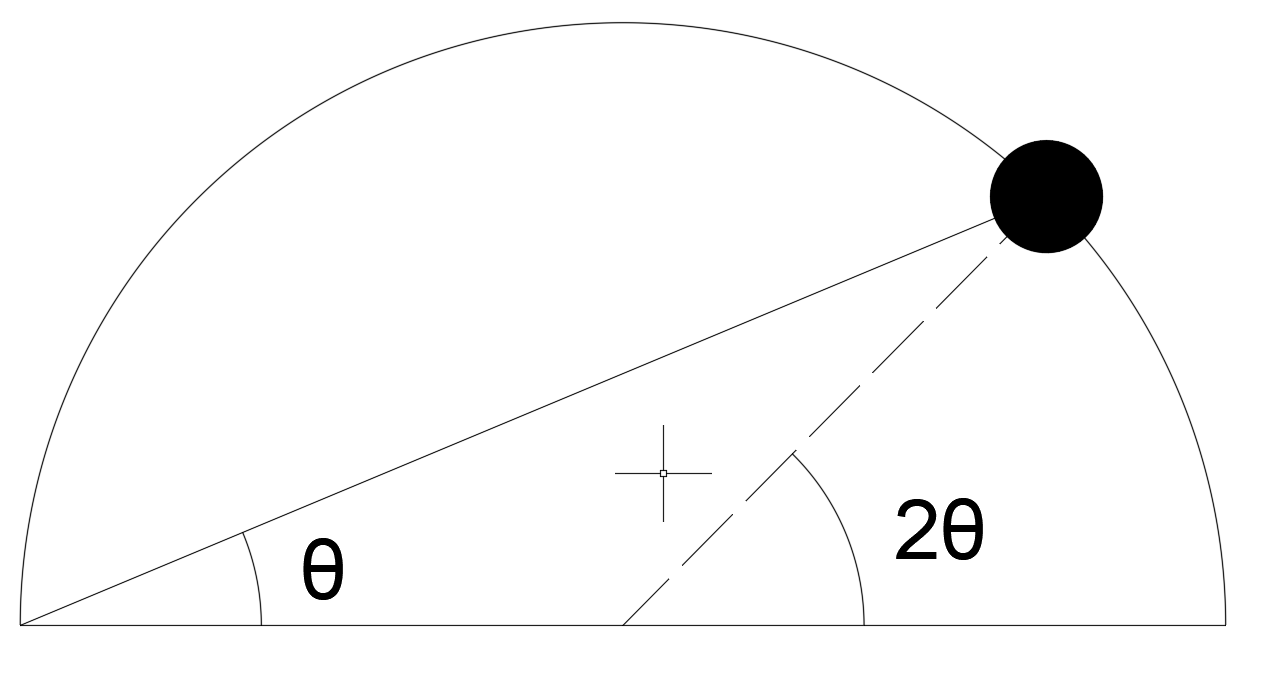
\includegraphics[height=100pt]{Chp2_illus1.png}
	\caption{练习20示意图}\label{fig:t20}
\end{figure}

\begin{align*}
A&=\int_{\theta=0}^{\theta=\frac{\pi}{4}}{\vec{F}}\cdot\di{\vec{x}}\\
&=\int_{\theta=0}^{\theta=\frac{\pi}{4}}F\di{x}\cos\left(\frac{\pi}{2}-\theta\right)\\
&=\int_{0}^{\frac{\pi}{4}}k(2R\cos\theta-0.1)\times\di{(R\times 2\theta)}\times\sin\theta\\
&=\int_{0}^{\frac{\pi}{4}}(-4R^2k\cos\theta+0.2Rk)\di{(\cos\theta)}\\
&=-2R^2k\cos^2\theta+0.2Rk\cos\theta\left.\right|_0^{\frac{\pi}{4}}\\
&=-2\times 0.2^2\times 40\times({\frac{\sqrt{2}}{2}}^2-1^2)+0.2\times 0.2\times 40\times(\frac{1}{2}-1)\\
&=0.8\sqrt{2}
\end{align*}


\section{计算题}
\exercise{21}

\solve 分别求解。

(1) 首先,有$\Delta l=\frac{F}{k}$,进而可得$E_p=\frac{1}{2}k(\Delta l)^2=\frac{F^2}{2k}$.由机械能守恒,可列出
$E_k-0=E_p-0$,代入各条件得
\[\frac{1}{2}Mv_{\text{右}}^2=\frac{F^2}{2k}\]
故得$v_{\text{右}}=\frac{F}{\sqrt{Mk}}$.

(2) 由受力分析知,$a_{\text{左}}=a_{\text{右}}$,即
\[\dy{v_{\text{左}}}{t}=-\dy{v_{\text{右}}}{t}\]
两边积分便得$v_{\text{左}}=-v_{\text{右}}+c$,代入刚恢复原长时的条件$v_{\text{左}}=0,v_{\text{右}}=\frac{F}{\sqrt{Mk}}$得
\[v_{\text{左}}+v_{\text{右}}=\frac{F}{\sqrt{Mk}}\]
故可见当$v_{\text{左}}=v_{\text{右}}$时,$v'_{\text{左}}=v'_{\text{右}}=\frac{F}{\sqrt{2Mk}}$。由机械能守恒可进一步得到
\[0+\frac{1}{2}M(v_{\text{右}})^2=\frac{1}{2}k(\Delta l)^2+\frac{1}{2}M(v'_{\text{左}})^2+\frac{1}{2}M(v'_{\text{右}})^2\]
解得$\Delta l=\pm\sqrt{\frac{M\left(\frac{F^2}{Mk}-2\times\frac{F^2}{4Mk}\right)}{k}}=\pm\frac{\sqrt{2}}{2}\frac{F}{k}$,即伸长或压缩$\frac{\sqrt{2}}{2}\frac{F}{k}$。

\exercise{22} 

\solve 记$x$为链条右端的位移,$l$为桌边链条的长度。据功的定义,有$\di{A}=F\cdot\di{x}=F\di{x}$;而当链条被匀速拉起,可知
\[F=G=M'g=\frac{l}{L}Mg\]
由几何意义,$\di{x}=-\di{l}$,故得
\[
A=\int_{\frac{L}{3}}^{0} -\frac{l}{L}Mg\di{l}
=\frac{Mg}{2L}l^2\left.\right|_{0}^{\frac{L}{3}}
=\frac{MgL}{18}
\]
如果有摩擦力$f$,则只需计算新的力
\[
F'=G+f=\frac{l}{L}Mg+\mu\left(\frac{L-l}{L}Mg\right)=\frac{Mg}{L}[\mu L+(1-\mu)l]
\]
进而就有
\begin{align*}
A&=\int_{\frac{L}{3}}^{0} -\frac{Mg}{L}[\mu L+(1-\mu)l] \di{l}=\frac{Mg}{L}\left.\left(\mu Ll+\frac{1-\mu}{2}l^2\right)\right|_{0}^{L/3}\\
&=\frac{Mg}{L}\left(\frac{\mu}{3}L^2+\frac{1-\mu}{18}L^2\right)=MgL\frac{5\mu +1}{18}
\end{align*}

\exercise{23}

\solve 首先,由图\ref{fig:t23-1},对小球应用牛顿第二定律:
\[m\dfrac{v^2}{R}=mg\cos\theta-N\]

\begin{figure}[htbp]
	\centering
	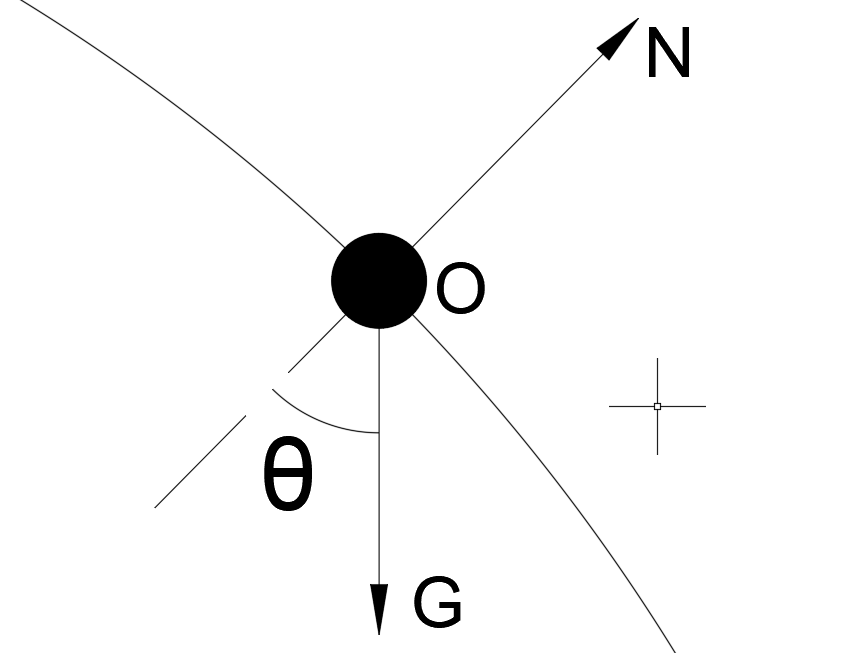
\includegraphics[height=100pt]{Chp2_illus2.png}
	\caption{练习23示意图1}\label{fig:t23-1}
\end{figure}

由受力分析(参见图\ref{fig:t23-2})知,圆环竖直方向受力$F$为
\[
F=(N'+N')\cos\theta=2N\cos\theta
\]

\begin{figure}[htbp]
	\centering
	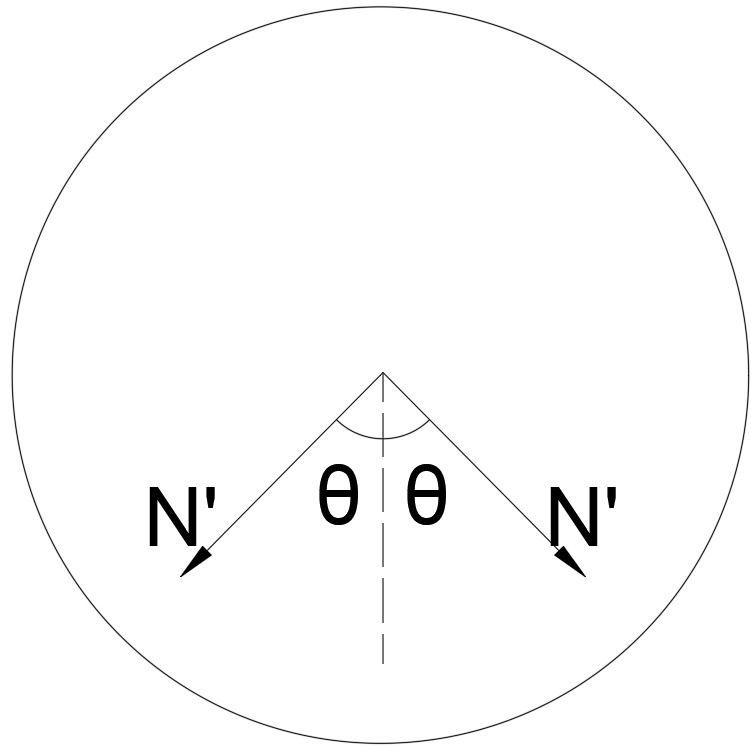
\includegraphics[height=100pt]{Chp2_illus3.png}
	\caption{练习23示意图2}\label{fig:t23-2}
\end{figure}

当$\theta\in[0,\frac{\pi}{2}]$时,$\cos\theta>0$,故当$N<0$时,$F$向上,圆环上升。从而有
\[N=mg\cos\theta-m\frac{v^2}{R}<0\]
由机械能守恒(见图\ref{fig:t23-3})得
\[\frac{1}{2}mv^2=mgh=mg(1-\cos\theta)R\]

\begin{figure}[htbp]
	\centering
	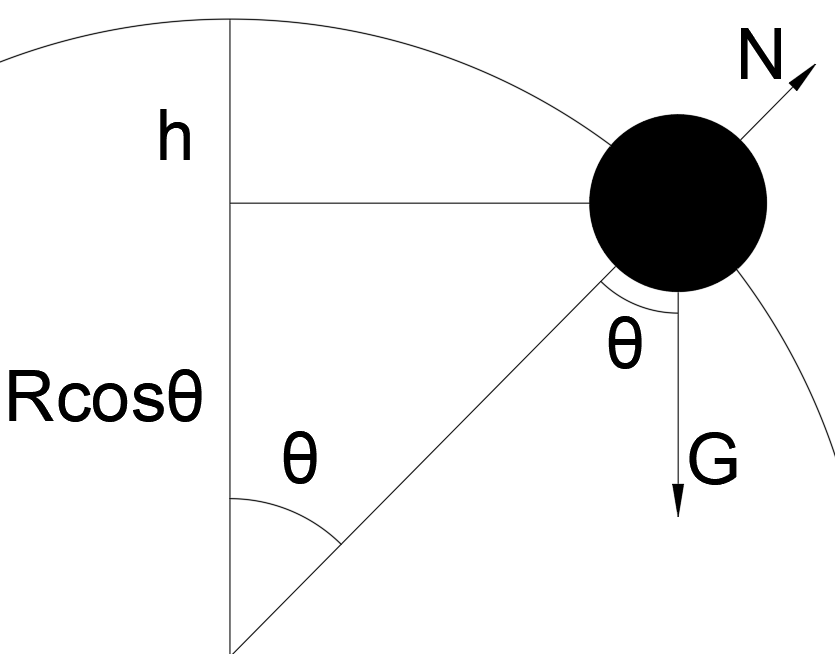
\includegraphics[height=100pt]{Chp2_illus4.png}
	\caption{练习23示意图3}\label{fig:t23-3}
\end{figure}

代入$N<0$的条件便得
\[mg\cos\theta-2mg(1-\cos\theta)<0\]
化简得$3\cos\theta<2$,解得$\theta>\arccos\frac{2}{3}$。即当$\theta>\arccos\frac{2}{3}$时,圆环会上升。

\exercise{24}

\solve $T_1$提供$G1+G2$,故有$k_1\Delta l=(m_1+m_2)g$,解得
\[\Delta l=\frac{(m_1+m_2)g}{k_1}\]
由机械能守恒有:
\[-mgx+\frac{1}{2}k_1(\Delta l+x)^2+\frac{1}{2}m_1v^2=0+\frac{1}{2}k_1(\Delta l)^2+0\]
解得
$v=\sqrt{\frac{-kx^2-2(k_1\Delta l-m_1g)x}{m_1}}=\sqrt{-\frac{k_1}{m_1}x^2-\frac{2m_2g}{m_1}x}$.利用二次函数最大值为$\frac{4ac-b^2}{4a}$的性质即得其最大值
\[
v_{\text{max}}=\sqrt{\frac{0-\frac{4m_2^2g^2}{m_1^2}}{4\left(-\frac{k_1}{m_1}\right)}}=\sqrt{\frac{m_2^2g^2}{m_1k_1}}=\frac{0.3\times 9.8}{\sqrt{0.5\times 8.9\times 10^4}}=0.0139(m/s)
\]



\chapter{功、能、冲量与动量}
\section{选择题}

\exercise{1}A

\solve 小球受到重力和弹簧弹力做的功,动能不守恒。小球受到的合外力不为0,因此动量不守恒。

\exercise{2}D

\solve 两船在过程中受到了人的摩擦力的作用,合外力不为零,动量不守恒。

\exercise{3}C

\solve 碰撞前后两球动量守恒,因此总动量为0,说明碰撞前两球动量大小相同,方向相反。

\exercise{4}D

\solve 两球碰撞后一起运动,说明为完全非弹性碰撞,存在机械能损失,因此机械能不守恒。两球还受到了弹簧弹力作用,合外力不为零,动量不守恒。

\exercise{5}D

\solve 运动半周前后小球的速度大小不变,方向相反,因此冲量大小\(I=m\Delta v=2mv=2mr \omega\)。

\exercise{6}C

\solve A人向右跳落入B船后,由动量守恒,A船具有向左的速度,A人具有向右的速度,落入B船后使得A人,B人,B船都具有了向右的速度。B人再跳回A船后,由动量守恒,B人获得的动量朝左,A人和B船获得的动量向右,因此最终B船的速度向右,\(v_B>0\)。B人和A船的动量都向左,因此最终B人落入A船后,A船速度向左,\(v_A<0\)。

\exercise{7}A

\solve 由公式\(E=\frac{p^2}{2m}\),\(p_1=\sqrt{2mE}\),\(p_2=\sqrt{2\times 4m\times E}=2\sqrt{2mE}\)(此处\(p_1\),\(p_2\)均为大小)。由于两个质点面对面运动,\(p_1\)和\(p_2\)符号相反,因此系统动量大小为\(p=p_2-p_1=\sqrt{2mE}\)。

\exercise{8}A

\solve 小球转一周后速度大小和方向都与转前相同,因此动量增量为0,A对。由冲量定义式\(I=F\Delta t\),\(F\)和\(\Delta t\)均不为0,因此\(I\)也不为0,B错,同理可知C错误。在转动过程中小球速度的方向发生了改变,因此过程中动量不守恒,D错。

\exercise{9}C

\solve 小球下落直到与板碰撞之前,对小球分析,有\(v=\sqrt{2gh}\),对板和弹簧分析,设此时弹簧的压缩量为\(x_0\),由胡克定律有\(x_0=Mg/k\);此后对球与板的碰撞过程,有动量守恒\(mv=(m+M)v_0\),解得\(v_0=\frac{m}{m+M}\sqrt{2gh}\);此后,小球与板一起运动,设两者一起运动的距离为\(x\),由能量守恒可列出
\[\frac{1}{2}(m+M)v_0^2+(M+m)gx+\frac{1}{2}kx_0^2=\frac{1}{2}k(x+x_0)^2\]
代入数据解得\(x=\frac{mg}{k}(1+\sqrt{1+\frac{2kh}{(M+m)g}})\),所以选择C项。

\exercise{10}A

\solve 两球碰撞后以相同速度运动,则为完全非弹性碰撞,必有机械能损失,与完全弹性碰撞矛盾,A错误;若两球碰撞前速度大小相同,方向相反,则碰撞后速度互换,B正确;完全弹性碰撞的定义即为机械能守恒的碰撞,C正确;碰撞过程中动量守恒,D正确。

\section{填空题}
\exercise{11}$10m/s$

\solve 以人和船为系统,过程中所受外力为$ 0 $,因此动量守恒。有
\begin{equation*}
(m+M)v=m(v'+\frac{v}{2})+M\frac{v}{2} 
\end{equation*}
代入数据解得$ v'=10m/s $.

\exercise{12}$ m\sqrt{2gh} $ \hspace{2em} 竖直向下

\solve $(1)$由$ I=\Delta p=F\Delta t $,小球下落时间为$\Delta t=\sqrt{\frac{2h}{g}}$,下落过程所受合外力为$F=mg$,故动量增量为
\begin{equation*}
\Delta p=mg\cdot\sqrt{2h/g}=m\sqrt{2gh}
\end{equation*}

$(2)$由合外力(重力)方向竖直向下,可得动量增量方向竖直向下。

\exercise{13}$\frac{5}{3}N\cdot s$,方向与力的方向同向 \hspace{2em} $\frac{5}{6}$N

\solve 由冲量定义,$I = \int F \di t$,对于本题来说,$F$是时间的函数,所以有
\begin{equation*}
I = \int_0^1 2t \di t + \int_1^2 2(2-t)^2 \di t = \frac{5}{3}\text{N} \cdot \text{s}
\end{equation*}
平均冲力为
\begin{equation*}
\overline{F} = \frac{I}{t} = \frac{5}{6} \text{N}.
\end{equation*}

\exercise{14}$-m\vec{v}$

\solve 对全过程,由动量定理,$\vec{I} = \Delta \vec{p} = -m\vec{v}$。

\exercise{15}$2350$kg$\cdot$ m/s \hspace{2em} 与炮弹飞行方向相反

\solve 由动量定理,$I = \Delta p = m(v-v_0)$,代入数据得$I=2350$kg$\cdot$ m/s,因为炮弹为减速运动,所以冲量方向与炮弹飞行方向相反。

\exercise{16}$\frac{m+M}{m}\sqrt{2 \mu gs}$

\solve 设子弹刚发射时的速度为$v_0$,子弹射入木块后共速速度为$v$。对子弹射入木块的过程,有动量守恒$mv_0=(M+m)v$,此后木块和子弹共同运动,由动能定理可列出
\begin{equation*}
\frac{1}{2}(m+M)v^2=\mu (m+M)gs
\end{equation*}
代入数据解得
\begin{equation*}
v_0=\frac{m+M}{m}\sqrt{2 \mu gs}.
\end{equation*}

\exercise{17}$\sqrt{\frac{kMl_0^2}{(M+m)^2}}$ \hspace{2em} $\sqrt{\frac{M}{M+nm}}l_0$

\analysis 每次油滴落入容器等价于油滴与容器发生了一次完全非弹性碰撞,该过程满足动量守恒;此后直到下一滴油滴落入容器之前,整体运动满足能量守恒。

\solve 当弹簧第一次达到原长即容器第一次到达滴管下方(第一滴油滴未滴入)时,设容器速度为$v_0$,由能量守恒
\begin{equation*}
\frac{1}{2}Mv_0^2=\frac{1}{2}kl_0^2
\end{equation*}
可得
\begin{equation*}
v_0=\sqrt{\frac{k}{M}}l_0
\end{equation*}
再设第$n$滴油滴滴入容器后容器与油滴整体的速度为$v_n$;由动量守恒$P_0=P_n$,其中初状态动量$P_0=Mv_0$,第$n$滴油滴滴入后动量$P_n=(M+nm)v_n$,解得
\begin{equation*}
v_n=\frac{M}{M+nm}v_0
\end{equation*}
此后容器达到偏离$O$点的最大运动距离$x_n$过程中,由能量守恒,有
\begin{equation*}
\frac{1}{2}(M+nm)v_n^2=\frac{1}{2}kx_n^2
\end{equation*}
成立,从中可解出
\begin{equation*}
x_n=\sqrt{\frac{M+nm}{k}}v_n
\end{equation*}

故当$n=1$时,
\begin{equation*}
v_1=\sqrt{\frac{kMl_0^2}{(M+m)^2}}
\end{equation*}
滴入$n$滴油滴后,容器偏离$O$点的最大距离为
\begin{equation*}
x_n=\sqrt{\frac{M}{M+nm}}l_0.
\end{equation*}

\exercise{18}$m(\alpha\sin(\omega t)\vec{i}-(\beta\cos(\omega t)-\beta)\vec{j})$

\solve 由已知条件$a_x=\omega\alpha\cos(\omega t),a_y=\omega\beta\sin(\omega t)$,所以$v_x=\int a_x\di t=\alpha\sin(\omega t)+C_1$,$v_y=\int a_y\di t=-\beta\cos(\omega t)+C_2$,又由初始条件$t=0$时,$vec{v}=0$,可得$C_1=0$,$C_2=\beta$,所以质点在任一时刻的动量$\vec{p}(t)=m(\alpha\sin(\omega t)\vec{i}-(\beta\cos(\omega t)-\beta)\vec{j})$。

\exercise{19}$mv/\Delta t$

\solve 由平均力计算公式可得$\overline{F}=\frac{I}{\Delta t}=\frac{mv}{\Delta t}$。

\exercise{20}$\frac{1}{6}m(2v_B-v_A)^2$

\solve 因为发生完全弹性碰撞,结合能量守恒,可得碰撞过程中系统动能最小的时刻为弹性势能最大的时刻,亦即A、B共速的时刻,设共速时速度为$v$,则设B运动的方向为正方向由动量守恒有$2mv_B-mv_A=3mv$,此时的动能为
\begin{equation*}
E_k=\frac{1}{2}\cdot 3mv^2=\frac{1}{6}m(2v_B-v_A)^2.
\end{equation*}

\section{计算题}
\exercise{21}

\analysis $(1)$动量定理$(2)$因为$\overline{F}>>G$,所以可以忽略重力,再由平均力公式可以求解。

\solve $(1)$由动量定理
\begin{equation*}
I=\Delta(mv)=m(v_2-v_1)=1.0\times(10+25)=35\mathrm{kg\cdot m/s}
\end{equation*}
方向竖直向上。

$(2)$设球对地面的平均冲力为$F$,地面对球的平均冲力为$F_0$。

对小球撞击地面的过程分析:因为$\overline{F_0}>>G$,所以可以忽略重力。由平均力计算公式得
\begin{equation*}
\overline{F_0}=\frac{I}{t}=\frac{35}{0.02}\mathrm{N}=1750\mathrm{N}
\end{equation*}
再由牛顿第三定律可得
\begin{equation*}
\overline{F}=\overline{F_0}=1750\mathrm{N}
\end{equation*}
方向竖直向下。

注:实际上最好还是不要忽略重力,因为在这里考虑重力也是可计算的。那么此时有
\begin{equation*}
\overline{F_0}-mg=\frac{I}{t}
\end{equation*}
再由牛顿第三定律可得
\begin{equation*}
\overline{F}=\overline{F_0}+mg=1759.8\footnote{注意$g$取9.8$\mathrm{N/s}^2$}\mathrm{N}
\end{equation*}
方向竖直向下。

\exercise{22}

\analysis 全过程可分为两部分:一是子弹嵌入木块过程,动量守恒,二是子弹木块整体沿斜面上滑,能量守恒。

\solve 子弹嵌入木块瞬间动量守恒,有
\begin{equation*}
mv=(m+M)v'
\end{equation*}
再由运动分解,木块速度可分解为垂直于斜面的速度和沿斜面方向的速度,因为木块此后被约束在斜面上运动,所以垂直于斜面的速度突变为$0$,即木块的运动速度为
\begin{equation*}
V=v'\cos\theta
\end{equation*}
对于木块和子弹的沿斜面上滑过程,有能量守恒
\begin{equation*}
\frac{1}{2}(m+M)V^2=(M+m)gl\sin\theta
\end{equation*}
联立上述三式可解得:
\begin{gather*}
V=\frac{mv\cos\theta}{M+m}\\
l=\frac{m^2v^2\cos^2\theta}{2(M+m)^2g\sin\theta}.
\end{gather*}

\exercise{23}

\analysis 对于碰撞问题可以从能量守恒动量守恒两方面考虑。

\noindent\textbf{证明}\ 设运动的小球为球1,质量为$m_1$,静止的小球为球2,质量为$m_2$,碰撞前球1的速度为$\vec{v}_0$,碰撞后球1、球2的速度分别为$\vec{v}_1$、$\vec{v}_2$,且有$\vec{v}_1$垂直于$\vec{v}_2$。

对碰撞过程,由能量守恒有:
\begin{equation*}
\frac{1}{2}m_1v_0^2=\frac{1}{2}m_1v_1^2+\frac{1}{2}m_2v_2^2
\end{equation*}
即
\begin{equation}\label{eq:c3-t23-1}
v_0^2=v_1^2+\frac{m_2}{m_1}v_2^2
\end{equation}
由动量守恒有:
\begin{equation*}
m_1\vec{v}_0=m_1\vec{v}_1+m_2\vec{v}_2
\end{equation*}
因为$\vec{v}_1$垂直于$\vec{v}_2$
所以由勾股定理可得
\begin{equation*}
m_1^2 v_1^2 + m_2^2 v_2^2 = m_1^2 v_0^2
\end{equation*}
\begin{equation}\label{eq:c3-t23-2}
v_0^2=v_1^2+\frac{m_2^2}{m_1^2}v_2^2
\end{equation}
$(\ref{eq:c3-t23-2})-(\ref{eq:c3-t23-1})$得
\begin{equation*}
\frac{m_2}{m_1}(\frac{m_2}{m_1}-1)v_2^2=0
\end{equation*}
因为$v_2^2 \ne 0$且$m_2 \ne 0$,所以有$m_2/m_1-1=0$,即$m_1=m_2$。由此得证。

\exercise{24}

\analysis 将尘埃与飞船共同作为研究对象,则系统动量守恒,从而得到通过$m$与$v$的关系,再通过$\di m$的表达式与前式联立可以消去$\di m$再积分得到$v$和$t$的关系

\solve 设$t$时刻飞船的质量为$m$,速度为$v$。由初末状态系统动量守恒,有$m_0 v_0=mv$,即
\begin{equation}
m=\frac{m_0 v_0}{v}
\end{equation}
对上式取微分,可得
\begin{equation}\label{eq:c3-t24-1}
\di m=- \frac{m_0 v_0}{v^2} \di v
\end{equation}
又有
\begin{equation}\label{eq:c3-t24-2}
\di m=\rho sv\di t
\end{equation}
$(\ref{eq:c3-t24-1})(\ref{eq:c3-t24-2})$两式联立消去$\di m$,再求积分,可得
\begin{equation*}
-\int_{v_0}^v \frac{\di v}{v^3}=\int_0^t \frac{\rho s}{m_0 v_0} \di t
\end{equation*}

解得$v=\sqrt{\frac{m_0}{2\rho sv_0 t+m_0}}v_0$.


\chapter{刚体运动学}
\note 笔者并不建议按照转动定理等名称记忆刚体运动的公式。实际上这些公式都是质点运动学各定律的延伸(如角动量对应动量,转动惯量对应质量,转动定理和动量矩定理对应牛顿第二定律等),做题的时候只需要认定该问题需要用质点运动学的哪些定律,再将质量,力等物理量换成刚体运动学中的转动惯量,力矩等即可。但为了与课本表述一致,在本解析中仍然按照刚体运动学公式名称引用,但会在其后附注数学表达式以方便对应。

\section{选择题}
\exercise{1}C

\solve 直观地理解,两个系统所受合外力均为$ Mg $,图A要驱动滑轮和重物(他们都获得了加速度),图B只需要驱动滑轮,因此$ \beta_A<\beta_B $。驱动滑轮的力为$ T_A $和$ T_B $,因此必有$ T_A<T_B $。

从定量计算来看,显然$ T_B=F=Mg $。对A滑轮,对物体应用牛顿第二定律$F=ma$,对滑轮应用转动定律$M=J\beta$:
\[Mg-T_A=Ma\]
\[T_A\times R=J\beta\]
与$ a=\beta R $联立解得:
\[T_A=\frac{Mg}{\frac{MR^2}{J}+1}\]
则有$ T_A< Mg=T_B$

\exercise{2}D

\solve 首先,此题讨论的是细棒对于$ O $点的转动惯量,如图\ref{fig:c4-t2}所示。由于细棒对于其一个端点的转动惯量恒为$ \frac{1}{3}ml^2 $,因此转动惯量不变。至于角加速度$ \beta $,由转动定律$M=J\beta$:
\[Mg\frac{l}{2}\sin\theta=\frac{1}{3}ml^2\times\beta\]
解得$ \beta=\frac{3Mg\sin\theta}{2ml} $,可知$ \beta $随下落过程中$ \theta $的减少而减少,因此角加速度从大到小。

\begin{figure}[htbp]
	\centering
	\begin{tikzpicture}
	\draw[dashed](0,0) -- (3,0);
	\draw[dashed](0,0) -- (0,-3);
	\draw[dashed](3,0) arc (0:-90:3);
	\draw(0,0) -- (2.4,-1.8);
	\draw(0.5,0) arc (0:-36.87:0.5) node[right=5pt] {$ \theta $};
	\end{tikzpicture}
	\caption{练习2示意图}\label{fig:c4-t2}
\end{figure}

\exercise{3}D

\solve 本题默认水平圆盘放在桌子上,力矩均指对轴的力矩。在玻璃球自由滚动的时候,系统受三个力:重力,支持力(与重力抵消,合力矩为0),还受轴对圆盘的支持力,但由于该力的$ \vec{r}=0 $,因此该力力矩也为0,合外力矩也为0。由动量矩定理$ M=\dy{L}{t} $知,此系统角动量守恒,D正确。若小球处于滚动状态,则轴对圆盘可能会有支持力的作用,由冲量定理$ (I=\Delta p) $,动量不守恒,A,B均错误。若小球与轴或者盘边缘碰撞,由于题目中未说明小球与轴或盘边缘的碰撞是否是完全弹性碰撞,因此碰撞可能会产生机械能损失,C错误。

\begin{note}
	笔者希望同学们对这类圆盘(或细棒)受到固定轴约束转动的问题有更多了解。轴对圆盘的力有且仅有两个,分别是摩擦力和支持力。对于支持力,其垂直于作用面,因此总是指向轴心,$ \vec{r}=0 $,该力对转轴的力矩为0。至于摩擦力,由于其与相对转动速度相反,因此该力与轴相切,由于轴是有半径的(不是一条线),因此$ \vec{r}=R $(R为转轴的半径,显然摩擦力的力矩不为0(但在碰撞过程中,由于$ \Delta t\to 0 $,由动量矩定理,该力矩导致的角动量变化$ \Delta L\to 0 $,因此也可认为角动量守恒)。该题中已经说明忽略轴的摩擦,因此圆盘和小球受到的合外力矩为0。更多相关内容请参考舒幼生著《力学(物理类)》
	\footnote{舒幼生. 力学: 物理类[M]. 北京大学出版社, 2005.}
	。
\end{note}

\exercise{4}C

\solve 角动量的定义为$ L=\vec{r}\times m\vec{v} $,$ m $为质点质量,$ \vec{v} $为质点速度(运动状态),$ \vec{r} $为质点的向径(与坐标原点有关),C正确,ABD均错误。

\exercise{5}D

\solve 参见图\ref{fig:c4-t5},微元$ \di{\sigma} $到轴的距离为$ x $。由于积分域关于$ x $轴对称,被积函数关于$ y $为偶函数,因此$ J=2J_1 $,$ J_1 $为第一象限部分的转动惯量。

\begin{figure}[htbp]
	\centering		
	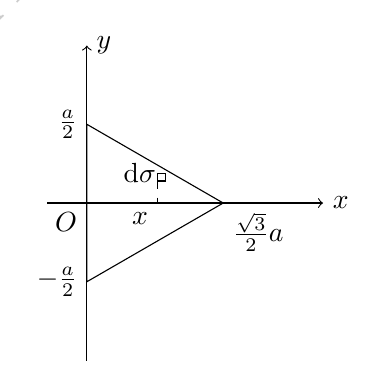
\begin{tikzpicture}
	\zbj{-0.5}{3}{-2}{2}
	\draw (0,-1) node[left] {$ -\frac{a}{2} $}
	-- (0,1) node[left] {$ \frac{a}{2} $}
	-- (1.732,0) node[below right] {$ \frac{\sqrt{3}}{2}a $}
	-- cycle;
	\draw [dashed](0.9,0.28) -- (0.9,0);
	\node[dashed,below left] at (0.9,0) {$ x $};
	\draw (0.9,0.280) rectangle (1,0.38) node [left]{$\di{\sigma}$};
	\end{tikzpicture}
	\caption{练习5示意图}\label{fig:c4-t5}
\end{figure}

按转动惯量之定义作积分,可得:
\begin{align*}
J&=2J_1=2\iint\limits_{\sigma_1}x^2\cdot\di{m}=2\iint\limits_{\sigma_1}x^2\cdot\left(m\frac{\di{\sigma}}{\frac{\sqrt{3}}{4}a^2}\right)\\
&=\frac{8m}{\sqrt{3}a^2}\int_0^{\frac{\sqrt{3}}{2}a}\di{x}\int_0^{\frac{1}{2}a-\frac{\sqrt{3}}{3}x}x^2\di{y}=\frac{8m}{\sqrt{3}a^2}\int_0^{\frac{\sqrt{3}}{2}a}\di{x}\left(\frac{1}{2}ax^2-\frac{\sqrt{3}}{3}x^3\right)\\
&=\frac{8m}{\sqrt{3}a^2}\left.\left(\frac{1}{6}ax^3-\frac{\sqrt{3}}{12}x^4\right)\right|_0^{\frac{\sqrt{3}}{2}a}=\frac{8m}{\sqrt{3}a^2}\left(\frac{\sqrt{3}}{16}a^4-\frac{3\sqrt{3}}{64}a^4\right)\\
&=\frac{8m}{\sqrt{3}a^2}\frac{\sqrt{3}}{64}a^4=\frac{1}{8}ma^2
\end{align*}

即$ J=\frac{1}{8}ma^2 $.

\exercise{6}A

\solve 直观上理解,$ \sigma(\theta) $在$ \theta=\frac{\pi}{2} $时最大,在$ \theta=0 $或$ \theta=\pi $时最小,此即球面质量更多地分布在赤道附近,两极附近质量面密度小。由于赤道附近距离$ z $轴距离更大,因此分布不均匀的球面转动惯量更大,A正确。\par
通过计算也可以得到相同的结论,此处不再赘述。

\exercise{7}A

\solve 碰撞过程中$ \Delta t\to 0 $,小球和系杆组成的系统受到4个力:重力,支持力(与重力相互抵消),O点对杆的支持力,O点对杆的摩擦力。因此系统角动量守恒(详细分析可见选择题3的“注”部分),有:
\[0+rmv=\left[\frac{1}{12}ml^2+m\left(\frac{l}{2}\right)\right]^2\omega\]
解得$\omega=\dfrac{3v}{2l}$.

\exercise{8}C

\begin{figure}[htbp]
	\centering
	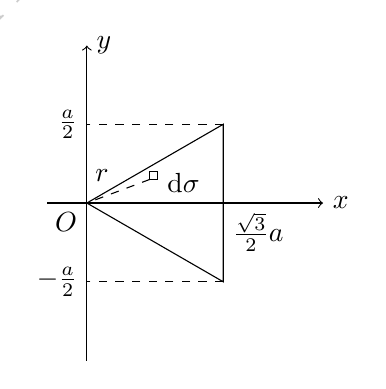
\begin{tikzpicture}
	\zbj{-0.5}{3}{-2}{2}
	\draw (0,0)-- (1.732,1) -- (1.732,-1) -- cycle;
	\draw[dashed] (1.732,1) -- (0,1) node[left] {$ \frac{a}{2} $};
	\draw[dashed] (1.732,-1) -- (0,-1) node[left] {$ -\frac{a}{2} $};
	\node[below right] at (1.732,0) {$\frac{\sqrt{3}}{2}a$};
	\draw (0.8,0.3) rectangle (0.9,0.4);
	\draw [dashed](0.8,0.3) -- node[above left] {$ r $} (0,0);
	\node [below right] at (0.9,0.5) {$\di{\sigma}$};
	\end{tikzpicture}
	\caption{练习8参考图}\label{fig:c4-t8}
\end{figure}

\solve 参考图\ref{fig:c4-t8},微元$ \di{\sigma} $到轴(就是到原点)的距离为$ \sqrt{x^2+y^2} $。由于积分域关于$ x $轴对称,被积函数关于$ y $为偶函数,因此$ J=2J_1 $,$ J_1 $为第一象限部分的转动惯量。则
\begin{align*}
J&=2J_1=2\iint\limits_{\sigma_1}\left(m\frac{\di{\sigma}}{\frac{\sqrt{3}}{4}a^2}\right)(x^2+y^2)\\
&=\frac{8m}{\sqrt{3}a^2}\int_0^{\frac{\sqrt{3}}{2}a}\di{x}\int_0^{\frac{\sqrt{3}}{3}x}(x^2+y^2)\di{y}
\end{align*}
进一步计算\footnote{可参考本章练习5中类似积分式的计算过程。}可得$ J=\frac{5}{12}ma^2 $.

\exercise{9}A

\solve 由动量矩定理易知A正确。BCD均为充分条件。小球在绳子的束缚下绕定点做匀速圆周运动,则所受合外力不为0(绳子的拉力),B错误,且小球受到的重力和支持力对定点的力矩均不为0,因此受到了外力矩的作用,C错误。对于D,可令$ J=t,\omega=\frac{1}{t} $,则$ L=J\omega=1 $,角动量守恒,但转动惯量和角速度都在随时间变化,因此D错误。

\exercise{10}A

\solve 卫星做匀速圆周运动,则$ m,v,r $均不变,$ \vec{r}\times\vec{v} $的方向也不变,因此角动量守恒。卫星与地球的万有引力与卫星的运动方向恒垂直,因此卫星与地球构成的系统的内力(万有引力)不做功,同时又不受外力作用,因此卫星的动能守恒。

\section{填空题}
\exercise{11}$\frac{3M}{ma} \hspace{2em} \frac{18M^2}{m^2a^3}t^2$

\solve 本题中转动方向固定,用标量形式计算即可。首先有
\[\beta=\frac{M}{J}=\frac{6M}{ma^2}\]
开始时$\omega=0$,故对$\beta$积分即可依次得到
\begin{gather*}
\omega=\frac{6M}{ma^2}t\\
v=\omega r=\frac{6M}{ma^2}t\times\frac{a}{2}=\frac{3M}{ma}t
\alpha_{\tau}=\dy{v}{t}=\frac{3M}{ma}\\
\alpha_n=\frac{v^2}{r}=\frac{\left(\frac{3M}{ma}t\right)^2}{\frac{a}{2}}=\frac{18M^2}{m^2a^3}t^2
\end{gather*}


\exercise{12}$\frac{1}{12}mR^2\omega_0^2$

\solve 圆柱所受合外力为摩擦力$f$,效果使得圆柱的质心运动速度$ v_c $增大。

圆柱所受合外力矩为摩擦力矩$ M_f $,效果使得圆柱的角速度$ \omega $减小。

圆柱做纯滚动的瞬间,即$ v_c=\omega R $。因此求得$ v_c $和$ \omega $对时间的函数,解出$ t $即可。

对圆柱使用牛顿第二定律$F=ma$和转动定律$M=J\beta$,可得
\[\begin{cases}
a_c=\dfrac{f}{m}=\mu g&\Rightarrow v_c=0+\mu gt=\mu gt\\[0.5cm]
\beta=\dfrac{M}{J}=\dfrac{-\mu mgR}{\dfrac{1}{2}mR^2}=-\dfrac{2\mu g}{R}&\Rightarrow\omega=\omega_0+\beta t=\omega_0-\dfrac{2\mu g}{R}t
\end{cases}\]
代入纯滚关系式,有
\[\mu gt=\omega_0R-2\mu gt\]
解得$t=\frac{\omega_0R}{3\mu g}$,此时
$v_c=\mu g\frac{\omega_0R}{3\mu g}=\frac{\omega_0R}{3}$,$\omega=\omega_0-\frac{2\mu g}{R}\frac{\omega_0R}{3\mu g}=\frac{\omega_0}{3}$。由柯尼希定理,可算得
\[E_{\text{总}}=\frac{1}{2}mv_c^2+\frac{1}{2}J\omega^2=\frac{1}{2}m\left(\frac{\omega_0R}{3}\right)^2+\frac{1}{2}\left(\frac{1}{2}mR^2\right)\left(\frac{\omega_0}{3}\right)^2=\frac{1}{12}mR^2\omega_0^2\]

\exercise{14}$\frac{1}{8}Mg$

\solve 物体加速度$ a $与滑轮角加速度$ \beta $的关系为:
\[\beta=\frac{a}{R}=\frac{g}{4R}\]
对滑轮应用转动定律$M=J\beta$:
\begin{gather*}
TR=\frac{1}{2}MR^2\beta\\
\therefore T=\frac{MR^2}{2R}\frac{g}{4R}=\frac{1}{8}Mg
\end{gather*}

\exercise{15}$\frac{1}{2l}\left(\sqrt{\frac{3gl}{2}}+\frac{v_0}{2}\right)$

\solve 首先计算碰撞前杆的角速度,由机械能守恒:
\begin{gather*}
0+0=Mg(-\frac{l}{2}\sin 30^\circ)+\frac{1}{2}J\omega^2\\
\omega_1=\sqrt{\frac{Mgl}{4}\frac{2}{\frac{1}{3}Ml^2}}=\sqrt{\frac{3g}{2l}}
\end{gather*}

以杆和子弹为系统,在碰撞过程中,所受外力里只有O点对杆的支持力为无穷大(抵消子弹沿杆方向的速度),但该力产生的力矩为0,因此碰撞过程中系统角动量守恒,有:
\begin{gather*}
l\sin 30^\circ mv_0+J\omega_1=(J+ml^2)\omega\\
\therefore \omega=\frac{1}{2l}\left(\sqrt{\frac{3gl}{2}}+\frac{v_0}{2}\right)
\end{gather*}

\exercise{16}$\frac{1}{4}mR^2$

\solve 均匀圆形薄板对圆心的转动惯量$ J=\frac{1}{2}mR^2 $,由垂直轴定理,$ J=J_1+J_2 $,$ J_1,J_2 $分别为薄板对其自身一条直径的转动惯量(两条相互垂直的直径)。由于圆板为圆对称,对任意一条直径的转动惯量相同,因此$ J_1=J_2 $,则$ J_1=\frac{1}{2}J=\frac{1}{4}mR^2 $

\exercise{17}$J_1=J_2$

\solve 记薄板对垂直于自身并穿过中心的轴的转动惯量为$ J $。

由对称性,薄板分别相对于两条对角线的转动惯量相等,均为$J_1$;分别相对过其中心且平行于一边的轴的转动惯量也相等,均为$J_2$,如图\ref{fig:c4-t17}所示。

\begin{figure}[htbp]
	\centering
	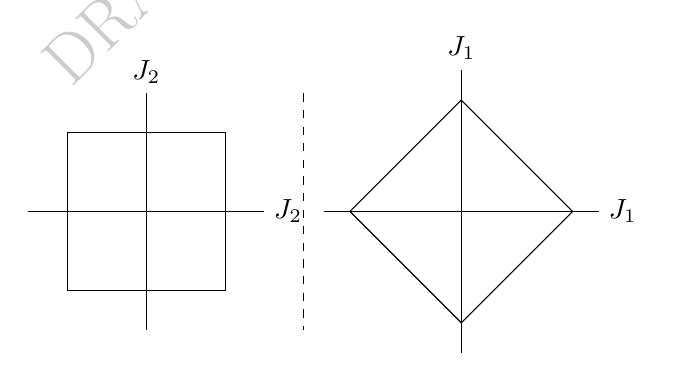
\begin{tikzpicture}
	\draw [rotate around={45:(4,0)}] (3,-1) rectangle (5,1);
	\draw (5.75,0) node[right] {$ J_1 $} -- (2.25,0);
	\draw (4,1.8) node[above] {$ J_1 $} -- (4,-1.8);
	\draw [dashed] (2,1.5) -- (2,-1.5);
	\draw (-1,-1) rectangle (1,1);
	\draw (1.5,0) node[right] {$ J_2 $} -- (-1.5,0);
	\draw (0,1.5) node[above] {$ J_2 $} -- (0,-1.5);
	\end{tikzpicture}
	\caption{练习17参考图}\label{fig:c4-t17}
\end{figure}

由垂直轴定理,$ J=2J_1=2J_2 $,因此$ J_1=J_2 $。

\exercise{18}75 rad/s

\solve 物块受到重力,支持力(相互抵消),绳的拉力。由于绳的向径与拉力的方向在同一条直线上,因此小物块所受合外力矩为0,角动量守恒。则:
\[(mR_1^2)\omega_0=(mR_2^2)\omega\]
解得$\omega=\frac{R_1^2}{R_2^2}\omega_0=\frac{0.5^2}{0.1^2}\times 3=75\ (\mathrm{rad/s})$。

\exercise{19}0

\solve 棒球沿直线飞行,则速度$ \vec{v} $的方向沿该直线,向径$ \vec{r} $的方向也沿该直线,因此角动量$ L=\vec{r}\times m\vec{v}=0 $。

\exercise{20}$2\sqrt{\frac{g\sin\theta}{3l}}$

\solve 由机械能守恒,可列出
\begin{gather*}
\hspace{1pt}2mg\left(\frac{l}{2}\sin\theta\right)+mg\left(-\frac{l}{2}\sin\theta\right)+0+0\\
=0+0+\frac{1}{2}\left(2m\left(\frac{l}{2}\right)^2\right)\omega^2+\frac{1}{2}\left(m\left(\frac{l}{2}\right)^2\right)\omega^2
\end{gather*}
解得$\omega=2\sqrt{\frac{g\sin\theta}{3l}}$。

\section{计算题}

\exercise{21}$\frac{m}{m+\frac{1}{2}M}\frac{Sg}{rl}$

\solve 对左端下垂链条应用牛顿第二定律$F=ma$,对上端链条和飞轮应用转动定律$M=J\beta$,右端下垂链条应用牛顿第二定律$F=ma$:
\begin{gather}
m\frac{l-\pi r+S}{2l}g-T_1=m\frac{l-\pi r+S}{2l}a\label{eq:c4-t21-1}\\
(T_1-T_2)r=\left(\frac{1}{2}Mr^2+m\frac{\pi r}{l}r^2\right)\beta\label{eq:c4-t21-2}\\
T_2-m\frac{l-\pi r-S}{2l}g=m\frac{l-\pi r-S}{2l}a\label{eq:c4-t21-3}
\end{gather}
代入$a=\beta r,(\ref{eq:c4-t21-1})+(\ref{eq:c4-t21-2})/r+(\ref{eq:c4-t21-3})$得:

\begin{align*}
m\frac{S}{l}g&=m\frac{l-\pi r}{l}\beta r+\left(\frac{1}{2}M+\frac{m\pi r}{l}\right)\beta r\\
&\left(m+\frac{1}{2}M\right)\beta r
\end{align*}
故$\beta=\frac{m}{m+\frac{1}{2}M}\frac{Sg}{rl}$.

\exercise{22}$a=\frac{2}{7}g$

\solve 人相对绳子加速度为0,绳子相对地面加速度为0,故人相对地面加速度为$a$。对人应用牛顿第二定律$F=ma$,对滑轮应用转动定律$M=J\beta$,对重物应用牛顿第二定律$F=ma$,可分别得到:
\begin{gather}
mg-T_1=ma\label{eq:c4-t22-1}\\
(T_1-T_2)R=\frac{1}{4}mR^2\alpha\label{eq:c4-t22-2}\\
T_2-\frac{1}{2}mg=\frac{1}{2}ma\label{eq:c4-t22-3}
\end{gather}
按$(\ref{eq:c4-t22-1})+\frac{(\ref{eq:c4-t22-2})}{R}+(\ref{eq:c4-t22-3})$合并三个等式,得
\begin{align*}
\frac{1}{2}mg&=\frac{3}{2}ma+\frac{1}{4}ma=\frac{7}{4}ma
\end{align*}
解得$a=\frac{2}{7}g.$

\exercise{23}$\Delta x=31.36m,\Delta\theta=78.4rad$

\solve 本解析取$ g=9.8m/s^2 $
\footnote{若取$g=10$m$/$s${}^2$,则相应的结果为$\Delta x=32m,\Delta\theta=80rad.$}
。以物体初始位置为原点,竖直向下为$x$轴建立坐标系。由能量守恒可得:
\[0+0+0=mg(-x)+\frac{1}{2}mv^2+\frac{1}{2}\left(\frac{1}{2}MR^2\right)\omega^2\]
即
\[gx=\frac{1}{2}v^2+\frac{1}{4}\frac{M}{m}v^2=\left(\dfrac12+\frac{M}{4m}\right)\cdot\left(\dy{x}{t}\right)^2\]
稍加变形得到
\[\sqrt\frac{g}{\frac{1}{2}+\frac{M}{4m}}\di{t}=\frac{\di{x}}{\sqrt{x}}\]
两边积分便得$\sqrt\frac{g}{\frac{1}{2}+\frac{M}{4m}}t=2\sqrt{x}+C$.代入$ t=0,x=0$可得$c=0$,故最终有
\[x=\frac{gt^2}{2+\frac{M}{m}}\]
代入$t=4$s,便得到
\begin{gather*}
\Delta x=x\left.\right|_{t=4}=\frac{16g}{2+\frac{15}{5}}=\frac{16}{5}g=31.36(\mathrm{m})\\
\Delta\theta=\left.\theta\right|_{t=4}=\frac{x}{R}=\frac{16g}{5\times 0.4}=8g=78.4(\mathrm{rad})
\end{gather*}

\note 这三道题是同一类型的问题,都可以用角动量定理和受力分析(如练习21、22)两种方法来求解。前者指的是,把系统中平动的链条、重物都看作都是转动的,写出其对滑轮转轴的角动量的表达式,用角动量定理解出角加速度,再求解其他物理量;后者则分别研究每一部分的转动或平动,分别列运动学基本方程,用角加速度和加速度的关系联系起来。但求解时可以发现,消去拉力后得到的就是角动量定理的表达式,而用第一种方法求拉力时,又要列出第二种方法的受力分析。所以说,两种方法本质是也一样的,如果只问与加速度有关的量就选用第一种。我们希望,读者在复习时,能使用角动量定理自己把以上三道题再做一遍,以体会其中深意,尤其是受力方向和角动量方向之区别,及所导致列式上的不同。如果要问诸如下降的距离等,也可采用练习23的解法,就可避过求加速度,也是一种好的思路。这是最基本的题型之一,问法相对固定,难度不大,老师希望通过这三道题来让同学们掌握这类题型。在2019年期末试题中,就有一道解答题是这个题型。

\exercise{24}$\frac{3m_2^2(v_1+v_2)^2}{m_1^2l\mu g}$

\solve 本题所述力矩,全部指对O点的力矩。

撞击前后瞬间,子弹和细棒组成的系统仅受O点支持力,因此合外力矩为0。由角动量守恒:
\[lm_2v_1+0=-lm_2v_2+\frac{1}{3}m_1l^2\omega\]
解得$\omega=\frac{3m_2(v_1+v_2)}{m_1l}$而摩擦力对O点力矩可计算为:
\[M=\int_{r=0}^{r=l}f\di{r}=\int_{r=0}^{r=l}\mu \di{m}g\di{r}=\int_0^l\mu gr\left(m_1\frac{\di{r}}{l}\right)=\frac{\mu m_1gl}{2}\]
又由于
\[M=J\dy{\omega}{t}=J\dy{\omega}{\theta}\dy{\theta}{t}=J\dy{\omega}{\theta}\omega\]
故有$\frac{M}{J}\di{\theta}=\omega\di{\omega}$。由$\theta=0$时$\omega=0$,对等式两边从$\theta=0$开始积分可得
\[\frac{M}{J}\theta=\frac{1}{2}\omega^2\]
故最终得到
\[\theta=\frac{\omega^2}{2}\frac{J}{M}=\frac{1}{2}\frac{9m_2^2(v_1+v_2)^2}{m_1^2l^2}\frac{\frac{1}{3}m_1l^2}{\frac{\mu m_1gl}{2}}=\frac{3m_2^2(v_1+v_2)^2}{\mu m_1^2gl}\]

\chapter{狭义相对论}  % 使用章节\chapter{}来做一级标题
\section{选择题}  % 选择题、填空题和解答题使用\section{}

\exercise{1}C  % 题号使用这个命令,会自动生成标记,注记后写主要答案

\solve
飞船系中看,光信号走过一个飞船长度,为$l_0=c\Delta t$,此长度换回地球系,由尺缩公式有$l=l_0\sqrt{1-\left(\frac{u}{c}\right)^2}$,所以在地球系中看,飞船尾部接收器和光信号相向运动,最后相遇,此过程的时间为$\Delta t'=\frac{l}{c+u}=\frac{l_0\sqrt{1-(\frac{u}{c})^2}}{c+u}=0.6\mu s$.

%% 空一行开始下一个题目
\exercise{2}A

\solve
因为该立方体是沿(体)对角线方向运动,所以在地面系中观察,体对角线方向上尺缩为原来的$\sqrt{1-(\frac{v}{c})^2}=0.8$倍,而其他方向的尺寸并未改变,所以,在地面系中看,它的体积为$V=0.8L^3$。

事实上,不管在什么方向上尺缩,体积的变化应该是一样的。如果不能理解,可以在垂直运动方向上将物体截成无限个薄片(就像微分那样),他们的底面积没有改变而高缩短为0.8倍,总体积也变为0.8倍。

\exercise{3}A

\solve
题中仅说了在$S$系中观察到一物体以$0.3c$的速度运动,并没有说速度的方向,所以可以假设该物体沿$x$轴正向运动或沿$x$轴负向运动,用速度变换求出在$S'$系中可能观测到的最大最小速度。得到速度范围为$\frac{4}{17}c<v<\frac{16}{23}c$,约为$0.24c<v<0.70c$。

严格的来说(假设坐标系是二维的),我们应该设物体在$S$系中速度方向与x轴正向夹角为$\theta$,则$S'$系中:(SI)
\begin{align*}
v_y&=0.3c\sin\theta\\
v_x&=\dfrac{0.3c\cos\theta-0.5c}{1-\frac{0.5c\cdot 0.3c\cos\theta}{c^2}}=c(\dfrac{1.5}{1-0.15\cos\theta}-2)\\
v&=\sqrt{v_x^2+v_y^2}\\
&=c\cdot \sqrt{(0.3\sin\theta)^2+{\big(\frac{0.3\cos\theta-0.5}{1-0.15\cos\theta}\big)}^2}
\end{align*}
可以研究该函数单调性,但手动计算过于麻烦,故作如下分析:

由于对称性,取$\theta\in[0,\pi]$。当$\theta$从$\pi$减小到$\frac{\pi}{2}$时,$v_y$增大,$v_x$绝对值减小;但当$\theta$从$\frac{\pi}{2}$减小到$0$时,$v_y$减小,$v_x$绝对值仍减小,可以确定$v$是单调递减的,所以计算此范围内$\frac{4}{17}c<v<\frac{\sqrt{13}}{6}c$,足以囊括B、C、D选项,所以可以选A了。

事实上,可以借助函数绘图软件,发现$v$一直是单调递减的。

\exercise{4}C

\solve
在$S$系和$S'$系中看都是同时发生的,即$\Delta t=\Delta t'=0$,由洛伦兹变换可得$\Delta x=0$,所以这两个事件发生地点的$x$坐标一定相同.

\exercise{5}C

\solve
本题为第一题的延续,所以地面系中看,飞船在此过程中飞行的时间为$\Delta t'=0.5\mu s$,飞行的速度为$u=0.6c$,飞行的距离为$s=u\Delta t'=90m$.

\exercise{6}A

\solve
在$S'$系中两个事件同地发生,满足钟缓的条件,所以有$\Delta t=\frac{\Delta t'}{\sqrt{1-(\frac{v}{c})^2}}$成立,从中解得$v=0.8c$.(有关尺缩钟缓的疑问可以参考qyxf推出的《狭义相对论不得不说的那些事》)

\exercise{7}C

\solve
由题目信息可得,$E=1.25E_0$,又有$E=\frac{E_0}{\sqrt{1-\beta^2}}$,两式联立可得$\beta=0.6$.

\exercise{8}B

\solve
(1)真空中的光速是目前所发现的自然界物体运动的最大速度;(2)狭义相对论有尺缩、钟缓、质量变大等结论;(3)根据洛伦兹变换,当$\Delta t=0$但$\Delta x$不为零时,$\Delta t'$不为零,即在$S$系同时发生的两个不同地事件在$S'$系中不同时发生;(4)根据钟缓的条件,相对观察者静止不动的参考系观测到的事件最短.

\exercise{9}C

\solve
设碰后的合粒子质量为$M$,运动速度为$v'$,碰撞过程中,有能量守恒:$\frac{m_0}{\sqrt{1-(\frac{v}{c})^2}}c^2+m_0c^2=\frac{M}{\sqrt{1-(\frac{v'}{c})^2}}c^2$,还有量守恒:$\frac{m_0}{\sqrt{1-(\frac{v'}{c})^2}}v=\frac{M}{\sqrt{1-(\frac{v'}{c})^2}}v'$,两式相除以约去比较复杂的因子,计算后得出$v'=\frac{c}{3}$.本题读者应注意,两个质量为$m_0$的粒子碰撞后,质量并不是$2m_0$,因为非弹性碰撞中能量有耗散,所以质量应设为$M$然后再求解.

\exercise{10}D

\solve 由于
\begin{equation*}
\overrightarrow{F}=\frac{\di \overrightarrow{p}}{\di t}=\frac{\di m\overrightarrow{v}}{\di t}=\frac{\di m}{\di t}\overrightarrow{v}+m\frac{\di\overrightarrow{v}}{\di t}=\frac{\di m}{\di t}\overrightarrow{v}+m\overrightarrow{a}
\end{equation*}
故质点的加速度和合外力可以不在同各一方向上,且加速度的大小不与合外力大小成正比.

\section{填空题}
\exercise{11} 相对的 \qquad 运动状态

\exercise{12} $=0.6m\qquad >0.6m$

\solve 简单公式应用。因为$A$和$B$两个飞船相向匀速运动,$A$、$B$两者相对运动速度恒定,所以从$A$观察$B$与从$B$观察$A$的洛伦兹变换具有等价形式,故$B$中测得$A$上的米尺长度与$A$测得$B$中的米尺长度应相等;地球上观测者看来,若在地面系中看$A$和$B$二者的运动速度均为$v$,则$A$看$B$的运动速度由速度变换公式可得应为$v'=\frac{v+v}{1+\frac{v^2}{c^2}}>v$,因为尺缩公式为$l=l_0\sqrt{1-(\frac{v}{c})^2}$,相对速度越大,尺缩效应越明显,所以地球上观测者观察到两船上的米尺长度都$>0.6m$.

\exercise{13} $\frac{\sqrt{3}}{2}c$

\solve
根据题目已知信息可得,$\frac{m_0}{\sqrt{1-(\frac{v}{c})^2}}c^2-m_0c^2=m_0c^2$,从中解得$v=\frac{\sqrt{3}}{2}c$.

\exercise{14} 如下三式
\begin{equation*}
u'_x=\frac{u_x\sqrt{1-(\frac{v}{c})^2}}{1-\frac{v}{c^2}u_y}\quad u'_y=\frac{u_y-v}{1-\frac{v}{c^2}u_y}\quad u'_z=\frac{u_z\sqrt{1-(\frac{v}{c})^2}}{1-\frac{v}{c^2}u_y}
\end{equation*}

\exercise{15} $c$

\solve
设这个粒子的动质量为$m$,则$E=mc^2$,$p=mc$,所以$\frac{E}{p}=c$.

\exercise{16} $0.8c$

\solve
根据速度变换,有$v=\frac{v'+u}{1+\frac{u}{c^2}v'}=0.8c$.

\exercise{17}一切物理定律在不同的惯性系中具有相同的表达形式.

\exercise{18}$15s \qquad 5s$

\solve
$\analysis$(1)地面系中看,两信号发出间隔过程飞船走了$0.8c\cdot3s$的路程,地面上观测到信号被接收的时间应为“信号传递到飞船时间”加上“飞船向地球返回接收信号的传递时间”,设信息传递的速度也为光速,所以一个信号从发出到地球观测到被接受所花费的时间为两倍的传递时间.所以,地面上的工作者观测到两信号被接受的时间间隔为
\begin{equation*}
\Delta t=2\cdot(\frac{s_2}{c-0.8c}-\frac{s_1}{c-0.8c})+3s=2\cdot\frac{0.8c\cdot3s}{c-0.8c}+3s=15s
\end{equation*}

(2)地面系中发射信号为同地时间,满足钟缓条件,所以在飞船系中观测到两信号发射的时间间隔为
\begin{equation*}
\Delta t=\frac{\Delta t_0}{\sqrt{1-(\frac{v}{c})^2}}=\frac{3s}{\sqrt{1-0.8^2}}=5\mathrm{s}
\end{equation*}

\exercise{19} $\frac{1-\alpha\beta^2}{\sqrt{1-\beta^2}}L$

\solve
方法一:利用洛伦兹变换
\begin{equation*}
\Delta x=\frac{\Delta x'+u\Delta t'}{\sqrt{1-\beta^2}}=\frac{-L+u\frac{L}{v}}{\sqrt{1-\beta^2}}
\end{equation*}

方法二:利用速度变换,子弹在$S$系中沿$x$轴负方向的速度为
\begin{equation*}
v_{S1}=\frac{u-v}{1-\frac{uv}{c^2}}
\end{equation*}
变换到正方向为
\begin{equation*}
v_S=-v_{S1}=\frac{v-u}{1-\frac{uv}{c^2}}
\end{equation*}
在$S$系中车厢的长度为
\begin{equation*}
L_S=L\sqrt{1-(\frac{u}{c})^2}
\end{equation*}
所以子弹在$S$系中通过的距离为
\begin{equation*}
l=\frac{L_S}{v_S+u}\cdot v_S=\frac{1-\alpha\beta^2}{\sqrt{1-\beta^2}}L
\end{equation*}

\exercise{20}$\tau=1.0\times10^{-5}$ s

\solve
满足钟缓条件,故
\begin{equation*}
\tau=\frac{\tau_0}{\sqrt{1-(\frac{v}{c})^2}}=\frac{2.0\times10^{-6}s}{\sqrt{1-0.98^2}}=1.0\times10^{-5}\ \mathrm{s}.
\end{equation*}


\section{计算题}
%21,22,24题对原作者代码有改动
\exercise{21}

\analysis
衰变问题可以看做发生完全非弹性碰撞后静止的逆过程,所以可以采用动量守恒、能量守恒联立方程组求解.

\solve 
设$\beta_p=\frac{v_p}{c},\beta_\pi=\frac{v_\pi}{c}$

能量守恒
\begin{equation*}
M_\Lambda c^2=M_pc^2+E_{kp}+M_\pi c^2+E_{k\pi}
\end{equation*}
动量守恒
\begin{equation*}
P_p=\frac{M_p}{\sqrt{1-\beta_p^2}}v_p=\frac{M_\pi}{\sqrt{1-\beta_\pi^2}}v_\pi=P_\pi
\end{equation*}
又有
\begin{align*}
E_{kp}=(\frac{M_p}{\sqrt{1-\beta_p^2}}-M_p)c^2\\
E_{k\pi}=(\frac{M_\pi}{\sqrt{1-\beta_\pi^2}}-M_\pi)c^2\\
P^2c^2=M^2c^4-M_0^2c^4
\end{align*}

联立解得$v_p=0.106c,v_\pi=0.584c$

所以可得$E_{kp}=5.35\ \mathrm{MeV},E_{k\pi}=32.35\ \mathrm{MeV}$.

\exercise{22}

\solve 
设$\beta=\frac{v}{c}$,根据洛伦兹变换有:
\begin{equation*}
\Delta x'=\frac{\Delta x-v\Delta t}{\sqrt{1-\beta^2}}
\end{equation*}

又由题意得$\Delta x'=0$

所以$v=\frac{\Delta x}{\Delta t}=5\times10^7m/s$.

\exercise{23}

\analysis
$S'$系相对于$S$系沿$x$轴正方向匀速运动,所以在$x$方向会发生尺缩,但是在$y$方向则不会,所以会产生在$S$系和$S'$系中观测到的角度不同的结果.

\solve
$S'$系中,细棒速率为
\begin{equation*}
u'=\frac{u-v}{1-\frac{uv}{c^2}}
\end{equation*}
设相对细棒静止的参考系为$S''$系,$S''$系中,细棒在坐标轴上的投影为$\Delta x'',\Delta y''$,$S'$系中的投影为$\Delta x',\Delta y'$,$S$系中的投影为$\Delta x,\Delta y$.

由洛伦兹变换,
\begin{align*}
\Delta x''=\frac{\Delta x'}{\sqrt{1-(\frac{u'}{c})^2}}=\frac{\Delta c}{\sqrt{1-(\frac{u}{c})^2}}\\\Delta y''=\Delta y'=\Delta y
\end{align*}
而
\begin{equation*}
\tan{\theta}=\frac{\Delta y}{\Delta x}\quad \tan{\theta'}=\frac{\Delta y'}{\Delta x'}
\end{equation*}
所以
\begin{equation*}
\frac{\tan{\theta}}{\tan{\theta'}}=\frac{\Delta x'}{\Delta x}=\frac{\sqrt{1-(\frac{u'}{c})^2}}{\sqrt{1-(\frac{u}{c})^2}}\Rightarrow u'^2=\frac{3}{4}c^2
\end{equation*}
当$u'=\frac{\sqrt{3}}{2}c$时,代入速度变换式中解得
\begin{equation*}
v=\frac{2(1-3\sqrt{3})}{13}c<0
\end{equation*}
因为惯性系$S'$向$x$轴正方向运动,所以舍去.

当$u'=-\frac{\sqrt{3}}{2}c$时,代入速度变换式中解得
\begin{equation*}
v=\frac{2(1+3\sqrt{3})}{13}c
\end{equation*}

\exercise{24}

\solve
相对于实验室参考系
\begin{equation*}
\tau=\frac{\tau_0}{\sqrt{1-(\frac{v}{c})^2}}
\end{equation*}
又由于$l=v\tau$,联立上式可得$v=\sqrt{\frac{225}{901}c}=0.5c$.

\chapter{静电场(一)}
\section{选择题}

\exercise{1}C

\solve
两极板间场强为$E=\dfrac{q}{\varepsilon_0S}$,但这是由两极板共同贡献而成。
研究两板间作用力时,一个为施力物体,一个为受力物体。
单个无穷大带电平板的场强为$E_0=\dfrac{q}{2\varepsilon_0S}$,即在板的同侧是匀强电场,故作用力为$F=E_0\cdot q$。

\exercise{2}D

\solve
取以O为圆心、$r,r+\Delta r$为内、外径的圆环面元,其上各点到通过圆心、垂直盘面的轴线上的任一点距离相等。
则:
\begin{gather*}
\Delta S=2\pi r\di{r}\\
\sigma=\dfrac{q}{\pi R^2}
\end{gather*}
故
\begin{equation*}
\di{q}=\sigma \Delta S=\dfrac{2q}{R^2}r\di{r}
\end{equation*}

\exercise{3}C

\solve
计算面积分即可。在这里$x=x_0$,$\vec{E}$与$S$垂直。
\begin{equation*}
\iint\limits_S \vec{E}\di{S}=bx_0\cdot S=x_0bS
\end{equation*}

\exercise{4}A

\solve
由高斯定理,$E=\dfrac{q}{4\pi\varepsilon_0 r^2}$,只与$q$有关。

\exercise{5}D

\solve
由高斯定理,通过闭合曲面$S$的电通量只与面内的电荷有关,故电通量不变;由电场强度的叠加原理知,$q$在P点产生的场强不变,但Q的改变。由于是矢量加法,场强一定会改变。

\exercise{6}C

\solve
由高斯定理:
\begin{align*}
E\cdot 4\pi r^2&=\dfrac{1}{\varepsilon_0}\int_0^r\rho\cdot 4\pi r^2\di{r}\\
&=\dfrac{4\pi b}{\varepsilon_0}\int_0^r e^{-kr}\di{r}\\
&=\dfrac{4\pi b}{\varepsilon_0 k}(1-e^{-kr})\\
\end{align*}
所以
\begin{gather*}
E=\dfrac{b}{\varepsilon_0 k}\dfrac{1-e^{-kr}}{r^2}\\
r=\dfrac{1}{k}\text{时,}E_1=\dfrac{b}{\varepsilon_0}\cdot k(1-e^{-1})\\
r=\dfrac{2}{k}\text{时,}E_2=\dfrac{b}{\varepsilon_0}\cdot \dfrac{k}{4}(1-e^{-2})
\end{gather*}
故
\begin{equation*}
E_2=\dfrac{1-e^{-2}}{4(1-e^{-1})}E_1\approx 0.34E_1
\end{equation*}

\exercise{7}D

\solve
简单定积分。以棒上远离场点的一端点为原点,指向场点的方向为$x$轴正方向。
\begin{align*}
E&=\int_{0}^{L}\dfrac{1}{4\pi \varepsilon_0}\dfrac{\lambda\di{x}}{{(r+\frac{L}{2}-x)}^2}\\
&=\dfrac{Q}{4\pi \varepsilon_0 L}\cdot \dfrac{1}{{r+\frac{L}{2}-x}}\bigg|_0^L\\
&=\dfrac{Q}{\pi \varepsilon_0(4r^2-L^2)}
\end{align*}

\exercise{8}B

\solve
由高斯定理知,$\sum q_{\text{内}}=0$,即净电荷为零,但不能说明高斯面$S$内任一点都没有电荷。

\exercise{9}D

\solve
题中所谓的“点”是一个固定的点,只不过刚开始在气球外,最后在气球内。如图\ref{fig:c6-t9}。注意气球是有厚度的!
\begin{figure}[!htbp]
	\centering
	\includegraphics[width=\textwidth]{Chp6_illus1.ai}
	\caption{练习9 气球膨胀}\label{fig:c6-t9}
\end{figure}
点在气球外时,球外场强不变;点在球壳中时,高斯面包围的电荷减小,场强减小;点在气球内时,场强为0。

\exercise{10}B

\solve
该系统可以看作是半径为$R_1$、电荷体密度为$\rho$的均匀带电球体和半径为$R_2$、电荷体密度为$-\rho$的均匀带电球体的组合。应用均匀带电球体内部电场强度的矢量式
\footnote{
	$E=
	\begin{cases}
	\dfrac{\rho}{3\varepsilon_0}\vec{r} & r\leqslant R,\\
	\dfrac{\rho R^3}{3\varepsilon_0 r^3}\vec{r} & r > R
	\end{cases}$
	
	标量式中,$r>R$时,$E=\dfrac{\rho R^3}{3\varepsilon_0 r^2}$。
}得:
\begin{align*}
E&=\dfrac{\rho}{3\varepsilon_0}\vec{r}_1+\dfrac{-\rho}{3\varepsilon_0}\vec{r}_2\\
&\text{($r_1,r_2$分别是$O_1,O_2$到场点的矢径)}\\
&=\dfrac{\rho}{3\varepsilon_0}(\vec{r}_1-\vec{r}_2)\\
&=\dfrac{\rho}{3\varepsilon_0}\overrightarrow{O_1O_2}
\end{align*}
即空腔内为匀强电场。

\section{填空题}

\exercise{11}$-\dfrac{2VR}{3r^2}$\quad 沿球心到该点的矢径向外

\solve
由电势的定义和均匀带电球体电场强度公式(见练习10脚注)得:
\[
0-V=\int_{0}^{R}\dfrac{\rho r}{3\varepsilon_0}\di{r}+\int_{R}^{+\infty}\dfrac{\rho R^3}{3\varepsilon_0 r^2}\di{r}
\]
整理得:
\[
V=-\dfrac{\rho R^2}{2\varepsilon_0}
\]
与场强公式对比即知:
\[
E=-\dfrac{2VR}{3r^2}
\]
由于$V<0$,可知球体带正电荷,故场强方向沿球心到该点的矢径向外。

\exercise{12}$\dfrac{\lambda_1\lambda_2}{2\pi \varepsilon_0}\ln\dfrac{a+l}{a}$\quad 沿有限长带电线指向无限长带电线(或在纸面上向左)

\solve
以两直线交点为原点(或有限长带电线左端点),远离无限长直线为$x$轴正方向,沿有限长带电线建立坐标系。

由无限长带电直线场强公式得:
\begin{align*}
F&=\int_{a}^{a+l}\dfrac{\lambda_1}{2\pi \varepsilon_0 x}\lambda_2\di{x}\\
&=\dfrac{\lambda_1\lambda_2}{2\pi \varepsilon_0}\ln\dfrac{a+l}{a}
\end{align*}
两线均带正电,故有限长带电线受力方向为$x$轴正向。注意题目问的是无限长带电线的受力,而且答题时不要引入“$x$轴”。

\exercise{13}$-\dfrac{\sigma a^2}{2\varepsilon_0}$\quad$\dfrac{\sigma a^2}{2\varepsilon_0}$\quad 0

\solve
情景参见本章练习3、练习5。注意此处考虑曲面的外侧为正向,内侧为负。

\exercise{14}0\quad $\dfrac{(Q+4a\lambda)}{\varepsilon_0}$

\solve
第一空由对称性易得。第二空使用高斯定理,$\sum q_{\text{内}}=Q+4a\cdot\lambda$。注意题目问的不是场强。

\exercise{15}$\dfrac{\sqrt{2}a}{2}$

\solve
如图\ref{fig:c6-t15},设$q_0$与$A$的连线和$AB$的夹角为$\theta$。由对称性,合力方向与$AB$平行。
\begin{figure}[!htbp]
	\centering
	\includegraphics[width=0.5\textwidth]{Chp6_illus2.ai}
	\caption{练习15 受力分析}\label{fig:c6-t15}
\end{figure}
\begin{align*}
E&=2\cdot \dfrac{1}{4\pi\varepsilon_0}\dfrac{qq_0}{r^2+a^2}\cos\theta\\
&=\dfrac{qq_0}{2\pi\varepsilon_0}\dfrac{r}{{(r^2+a^2)}^{\frac{3}{2}}}
\end{align*}
令$f(r)=\dfrac{r}{{(r^2+a^2)}^{3/2}}$,则$f'(r)=\dfrac{a^2-2r^2}{{(r^2+a^2)}^{5/2}}$。
由导数知识得:$a^2-2r^2=0\text{即}r=\dfrac{\sqrt{2}}{2}a$时,$f(r)$取得极大值。

或者用三角换元。令$r=a\tan\theta$,则
\begin{gather*}
f(\theta)=\dfrac{1}{a^2}\sin\theta\cos^2\theta\\
f'(\theta)=\dfrac{1}{a^2}\cos\theta(\cos^2\theta-2\sin^2\theta)
\end{gather*}
由导数知识得:$\tan\theta=\dfrac{\sqrt{2}}{2}\text{即}r=\dfrac{\sqrt{2}}{2}a$时,$f(\theta)$取得极大值。

\exercise{16}$\dfrac{\sigma^2\Delta S}{2\varepsilon_0}$

\solve
均匀带电球面在其表面处产生的电场强度为
\[
E=\dfrac{\sigma\cdot 4\pi R^2}{4\pi\varepsilon_0R^2}=\dfrac{\sigma}{\varepsilon_0}
\]
但该电场也是由所取的面元和剩余部分共同贡献而成(同练习1),故作如下分析:

\begin{figure}[!htbp]
	\centering
	\includegraphics[width=0.5\textwidth]{Chp6_illus3.ai}
	\caption{练习16 场强分布}\label{fig:c6-t16}
\end{figure}
如图\ref{fig:c6-t16},红色部分为$\Delta S$,我们分球壳内外来研究。剩余部分球壳在$\Delta S$内、外侧(无限接近$\Delta S$且对称的)两点P、Q处产生的场强均可看作是$E_0$,而$\Delta S$在P、Q处产生的场强$E_1=E_2$。那么由题意知:
\begin{gather*}
\text{(P点)}E_0-E_1=0\\
\text{(Q点)}E_0+E_1=E\\
\end{gather*}
解得:
\[
E_0=E_1=\dfrac{1}{2}E=\dfrac{\sigma}{2\varepsilon_0}
\]
那么
\begin{gather*}
q_S=\sigma\Delta S\\
F=E_0q_S=\dfrac{\sigma^2\Delta S}{2\varepsilon_0}
\end{gather*}

\exercise{17}$-\dfrac{\lambda}{2\pi\varepsilon_0R}\vec{j}$

\solve
\[
\di{E}=\dfrac{\lambda \di{s}}{4\pi \varepsilon_0 R^2}=\dfrac{\lambda \di{\theta}}{4\pi \varepsilon_0 R}
\]
注意到电场强度是由圆环指向O点,故:
\[
\di{E_x}=\di{E}\cdot (-\cos\theta),\di{E_y}=\di{E}\cdot (-\sin\theta)
\]
积分\footnote{此后因对称性而场强为零的情景,不再积分计算。}得:
\begin{gather*}
E_x=\dfrac{\lambda}{4\pi \varepsilon_0 R}\int_0^{\pi} -\cos\theta\di{\theta}=0\\
E_y=\dfrac{\lambda}{4\pi \varepsilon_0 R}\int_0^{\pi} -\sin\theta\di{\theta}=-\dfrac{\lambda}{2\pi\varepsilon_0R}
\end{gather*}
故得$E=-\dfrac{\lambda}{2\pi\varepsilon_0R}\vec{j}$

\exercise{18}$\dfrac{\vec{p}}{2\pi\varepsilon_0x^3}$

\solve
设电偶极子的两电荷电量为$q$,距离为$l$。
\begin{align*}
E&=\dfrac{q}{4\pi\varepsilon_0}\cdot \dfrac{1}{(x-\frac{l}{2})^2}+\dfrac{-q}{4\pi\varepsilon_0}\cdot \dfrac{1}{(x+\frac{l}{2})^2}\\
&=\dfrac{q}{2\pi\varepsilon_0}\dfrac{xl}{{(x^2-\frac{l^2}{4})}^2}
\end{align*}
$x\gg l$时,$x^2-\dfrac{l^2}{4}\approx x^2$。同时考虑方向,可以得到:
\begin{align*}
E&=\dfrac{q\vec{l}}{2\pi\varepsilon_0x^3}\\
&=\dfrac{\vec{p}}{2\pi\varepsilon_0x^3}
\end{align*}

\exercise{19}0

\solve
复习高斯定理。

\exercise{20}$\dfrac{\lambda d}{\pi\varepsilon_0 a^2}$\quad 从O点指向细线端点连线中点

\solve
使用补偿法即可。而且$d\ll a$,故将空缺处看作点电荷。
\[
E=\dfrac{\lambda d}{4\pi\varepsilon_0{(\frac{a}{2})}^2}=\dfrac{\lambda d}{\pi\varepsilon_0 a^2}
\]
空缺了一些产生向下场强的电荷,故场强方向向上。

\section{解答题}

\exercise{21}

\solve
以O为极点,建立如图\ref{fig:c6-t21}所示的坐标系。极轴穿过圆弧的终点。
\begin{figure}[!htbp]
	\centering
	\includegraphics[width=0.5\textwidth]{Chp6_illus4.ai}
	\caption{练习21 坐标系}\label{fig:c6-t21}
\end{figure}
把柱面分成无限根无限长直导线(沿母线方向),设无限长导线长度为$l$,则其线密度$\lambda=\dfrac{\di{q}}{l}=\dfrac{\di{(\sigma l\cdot R\theta)}}{l}=\sigma R\di{\theta}$,故有
\[\di{E}=\dfrac{\lambda}{2\pi\varepsilon_0R}=\dfrac{\sigma}{2\pi\varepsilon_0}\di{\theta}\]
再由$\di{E_x}=-\di{E}\cos\theta,\di{E_y}=-\di{E}\sin\theta$可进一步求得:
\begin{gather*}
E_x=\dfrac{\sigma}{2\pi\varepsilon_0}\int_{-\frac{\theta}{2}}^{\frac{\theta}{2}}-\cos\theta\di{\theta}=-\dfrac{\sigma\sin\frac{\theta}{2}}{\pi\varepsilon_0}\\
E_y=\dfrac{\sigma}{2\pi\varepsilon_0}\int_{-\frac{\theta}{2}}^{\frac{\theta}{2}}-\sin\theta\di{\theta}=0
\end{gather*}
故所求场强大小为$\dfrac{\sigma\sin\frac{\theta}{2}}{\pi\varepsilon_0}$。

\exercise{22}

\solve
由对称性,场强方向沿$x$轴。取面积微元(见练习2),则:
\begin{align*}
E=&\int_0^R\dfrac{1}{4\pi\varepsilon_0}\cdot\dfrac{\frac{\sigma_0r}{R}\cdot 2\pi r\di{r}}{r^2+x^2}\cdot\dfrac{x}{\sqrt{r^2+x^2}}\\
&=\dfrac{\sigma_0x}{2\varepsilon_0R}\int_0^R\dfrac{r^2\di{r}}{{(r^2+x^2)}^\frac{3}{2}}\\
&=\dfrac{\sigma_0x}{2\varepsilon_0R}[-\dfrac{r}{\sqrt{r^2+x^2}}+\ln(r+\sqrt{r^2+x^2})]\Big|_0^R\\
&=\dfrac{\sigma_0x}{2\varepsilon_0R}\big(\ln\dfrac{R+\sqrt{R^2+x^2}}{x}-\dfrac{R}{\sqrt{R^2+x^2}}\big)
\end{align*}
方向沿$x$轴正向。

\exercise{23}

\solve
由题,取半径为$r(R_1<r<R_2)$的球面为高斯面。由高斯定理:
\begin{equation*}
E\cdot 4\pi r^2=\dfrac{1}{\varepsilon_0}(Q+\int_{R_1}^r\dfrac{A}{r}\cdot 4\pi r^2\di{r})
\end{equation*}
计算得:
\begin{equation*}
E=\dfrac{A}{2\varepsilon_0}+\dfrac{Q-2\pi AR_1^2}{4\pi r^2\varepsilon_0}
\end{equation*}
题目中$E$与$r$无关,故:
\begin{gather*}
Q-2\pi AR_1^2=0\\
A=\dfrac{Q}{2\pi R_1^2}
\end{gather*}

\exercise{24}

\solve
由对称性,场强方向沿$z$轴。以垂直于$z$轴的平面去截球壳得到小圆,取以该圆周长$2\pi R\sin\theta$为长、$R\di{\theta}$为宽的面元,可得(注意代入$\sigma_0$):
\begin{align*}
\di{E}&=\dfrac{\sigma_0\cdot 2\pi R\sin \theta R\di{\theta}}{4\pi \varepsilon_0 R^2}\\
&=\dfrac{\sigma}{2\varepsilon_0}\sin\theta\cos\theta\di{\theta}\\
E_z&=\int_0^{\frac{\pi}{2}}\di{E}\cdot(-\cos\theta)\di{\theta}\\
&=-\dfrac{\sigma_0}{2\varepsilon_0}\int_0^{\frac{\pi}{2}}\sin\theta\cos^2\theta\di{\theta}\\
&=-\dfrac{\sigma_0}{6\varepsilon_0}
\end{align*}
因此所求电场强度为$\dfrac{\sigma_0}{6\varepsilon_0}$,方向沿$z$轴负方向。

\chapter{静电场(二)} 
\section{选择题} 

\exercise{1}B 

\solve
两个平板之间的电场为匀强电场,若记向右为正方向,则电场强度:
\[E=\frac{\sigma}{2\epsilon_0}-\frac{2\sigma}{2\epsilon_0}=-\frac{\sigma}{2\epsilon_0}\]

即电场强度向左,电场线也指向左。由于电势沿着电场线降低,因此$V_B>V_A$。

\exercise{2}B

\solve 加入电介质之前,$ C_1,C_2 $电容相同,由于并联,则$ U $也相同,由电容定义$ C=\frac{Q}{U} $,两个电容器所带电荷$ Q_1=Q_2 $。

由于电键断开,因此电容器与外界没有电荷交换,过程中两个电容器的总带电量$ Q=Q_1'+Q_2' $不变。
插入电介质稳定后,相连的极板电势差应为$ 0 $(否则电荷会顺着电势减小的方向移动),则求$ C_1,C_2 $的电势差:
\[\Delta u'=\frac{Q_1'}{C\epsilon_r}=\frac{Q_2'}{C}\]

有:$Q_1'=\epsilon_r Q_2'$,因此$Q_2'<Q_2$,有电荷从$C_2$流向$C_1$,知$C_1$电量增大。

又因为$\Delta u'<\Delta u$,有$E'd<Ed$,$d$不变,可知场强变小,因此选B。

\note 做此类电容题目需要寻找过程中的不变量,若电容器的大小、形状等不变,则过程中电容$ C $不变;若电容器与外界没有电荷交换,则电量$ Q $不变。

\exercise{3}D

\solve A,电位移矢量会受到束缚电荷的影响,书上写道,若电介质是各向异性的,则$ D $与$ E $的方向可不一样。

B,电位移先起始于自由正电荷,终止于自由负电荷,不形成闭合线,不中断。

C,电位移线可以出现在真空中,此时电位移线与电场线相同。

D正确,由电介质中高斯定理可直接得到。

\exercise{4}D

\solve 两板间为匀强电场,电场强度大小为:
\[E=\left|\frac{-\sigma}{2\epsilon_0}-\frac{-2\sigma}{2\epsilon_0}\right|=\frac{\sigma}{2\epsilon_0}\]

则电势差大小:
\[\Delta u=Ed=\frac{\sigma d}{2\epsilon_0}\]

\exercise{5}C

\solve A,放入$q_2$之前球外场强关于O是球对称的,而$q_2$产生的电场关于$O$不是球对称的,由电场叠加原理,放入$q_2$后两个电场叠加,关于$O$不是球对称的,因此A错。

B,由静电屏蔽,$q_2$在外球壳内部产生的电场强度被外球壳的电荷所抵消,则导体内部的电场强度仅受到$q$和内表面上电荷的影响。由于$q$产生的电场关于$O$球对称,导体内部的电场强度由于静电平衡,均为$0$,也是关于$O$球对称,那么内表面电荷分布也必然是球对称,B错。

C,由于静电平衡,导体内部是等势体,自然内外表面电势差恒为$0$,C对。

D,$ q_1,q_2 $之间的静电作用力即使库仑力,大小为$ F_c=\frac{1}{4\pi\epsilon_0}\frac{q_1q_2}{r^2} $,显然不为0,D错。

\exercise{6}B

\solve 设均带有$ Q $的电荷,半径为$ R $和$ 2R $。则孤立导体球的电势为:$U_1=\frac{Q}{4\pi\epsilon_0R} $,$ U_2=\frac{Q}{8\pi\epsilon_0R} $,有$ U_1:U_2=2:1 $。而电场能量$ W=\frac{QU}{2} $,则可知$ W_1=W_2 $。

\exercise{7}C

\solve 电容与导体带电情况无关,因此电荷面密度$ \sigma $变化前后C不变,而$ Q_1:Q_2=1:2 $。由$ W=\frac{Q^2}{2C} $,则$ W_1:W_2=1:4 $,电场能量变为原来了的4倍。

\exercise{8}D

\solve 由电介质定义式,$ E=\frac{E_0}{\epsilon_r} $,$ E_0 $为自由电荷的贡献。而电场强度可拆分为自由电荷与束缚电荷的贡献之和,有$ E=E_0-E_r $。联立两式,消去$ E_0 $,得到$ E_r=(\epsilon_r-1)E $。

\exercise{9}C

\solve 由高斯定理,$P$点所在球面仍然只包含$ +q $电荷,因此电场强度不变。事实上,同理可知$r$-$R$之间的电场强度也不变。但对于R之外的电场强度,由高斯定理,大球面外包含的电荷为$ Q+q $,比加入球面之前$ (+q) $大,因此球面外的场强变大。因此对于整个空间上的任意一点,有$ E_2>=E_1 $。

由电势计算式,$ u=\int_a^{+\infty} E\cdot\di{l} $,由定积分的大小性质,有$ u_2>u_1 $,可见电势也增大。

\exercise{10}A

\solve 电容与电容器带电情况无关,因此变化前后电容不变,记为$ C $。

并联之前,充电的电容器电场能量$ W=\frac{Q^2}{2C} $,并联之后,两个电容器电势差相同。

由$ Q=CU $知带电量相同,又因为与外界没有电荷交换,则总带电量相同。则每个电容器电荷量为$ \frac{Q}{2} $。

总电场能量为$ W=2\times \frac{Q^2}{8C}=\frac{Q^2}{4C} $,有$ W_1:W_2=2:1 $,静电能减小。

\section{填空题}
\exercise{11} $4\pi\epsilon_0\epsilon_r\frac{R_1R_2}{R_2-R_1}$

\solve 见教材P149 例6.32,积分时不考虑$E_2$即可。

\exercise{12} $\frac{Q}{4\pi\epsilon_0 R}$ \quad $-\frac{Qq}{4\pi\epsilon_0 R}$

\solve 点电荷在一点产生的电势(见课本)为:
\[u=\frac{q}{4\pi\epsilon_0 R}\]

此处可将半圆形微元$R\di{\alpha}$视为点电荷,在O点产生的电势为:

\[\di{u}=\frac{R\di{\alpha}\lambda_0\sin\alpha}{4\pi\epsilon_0 R}\]

积分可得:
\begin{align*}
u&=\int_{\alpha=0}^{\alpha=\pi} \di{u}\\
&=\int_0^{\pi} \frac{R\di{\alpha}\lambda_0\sin\alpha}{4\pi\epsilon_0 R}\\
&=\frac{\lambda_0}{2\pi\epsilon_0}
\end{align*}

或由于微元到$O$点距离相同,直接用$Q$作为总电量写为$\frac{Q}{4\pi\epsilon_0 R}$即可。

当取无穷远处为电势零点时,$ u $表示将单位点电荷移动到无穷远处的过程中,电场力做的功,因此此处需要取负号,并乘$q$即可。

\exercise{13} $\frac{Q}{4\pi\epsilon_0\epsilon}\left(\frac{1}{R_1}+\frac{\epsilon-1}{R_2}\right)$

\solve 当金属球静电平衡时,电荷集中分布在球面上。由高斯定理可求出电场分布:

\begin{equation}
E=\left\{
\begin{aligned}
&\frac{Q}{4\pi\epsilon_0 r^2}\quad &R_2\leqslant r\\
&\frac{Q}{4\pi\epsilon r^2}\quad &R_1\leqslant r<R_2\\
&0	&r<R_1
\end{aligned}
\right.
\end{equation}

则$ P $点电势为:

\begin{align*}
u&=\int_r^{+\infty}E\cdot\di{r}\\
&=\int_r^{R_1}E\cdot\di{r}+\int_{R_1}^{R_2}E\cdot\di{r}+\int_{R_2}^{+\infty}E\cdot\di{r}\\
&=0+\frac{Q}{4\pi\epsilon_0 R_2}+\frac{Q}{4\pi\epsilon}\left(\frac{1}{R_1}-\frac{1}{R_2}\right)\\
&=\frac{Q}{4\pi\epsilon}\left(\frac{1}{R_1}+\frac{\epsilon-\epsilon_0}{\epsilon_0R_2}\right)
\end{align*}

\exercise{14} $1:1$

\solve 由电介质中的高斯定理,在$ Q $和$ S $都不变的情况下,$ D $也相同。

\exercise{15} $\frac{q}{4\pi \epsilon_0 r_1^2}$ \quad $\frac{q+Q}{4\pi\epsilon_0 r_2^2}$ \quad $\frac{1}{4\pi\epsilon_0}\left(\frac{q}{r_1}+\frac{Q}{R_2}-\frac{q+Q}{r_2}\right)$

\solve 由高斯定理计算得到电场强度:
\begin{equation}
E=\left\{
\begin{aligned}
&\frac{Q}{4\pi\epsilon_0 r^2}\quad &R_2\leqslant r\\
&\frac{q+Q}{4\pi\epsilon_0 r^2}\quad &R_1\leqslant r<R_2\\
&0	&r<R_1
\end{aligned}
\right.
\end{equation}

将A,B离O点的距离$ r_1,r_2 $代入即可得到场强大小。

而电势差则需要积分,积分路径为:A-OA连线与外球壳交点-沿外球壳移动到OB与外球壳交点-沿OB到B。球壳为等势面,因此在球壳上移动电场力做功为0。则电势差:
\begin{align*}
\Delta u&=\int_{r_1}^{R_2}E\cdot\di{r}+0+\int_{R_2}^{r_2}E\cdot\di{r}\\
&=\frac{q}{4\pi\epsilon_0}\left(\frac{1}{r_1}-\frac{1}{R_2}\right)+\frac{q+Q}{4\pi\epsilon_0}\left(\frac{1}{R_2}-\frac{1}{r_2}\right)\\
&=\frac{1}{4\pi\epsilon_0}\left(\frac{q}{r_1}+\frac{Q}{R_2}-\frac{q+Q}{r_2}\right)
\end{align*}

\exercise{16} 尖端放电

\exercise{17} $ -\frac{1}{12\pi\epsilon_0 R(3Q+q)} $

\solve 静电平衡时,金属球的电荷全部分布在表面上,且整个金属球为一个等势体,因此求出金属球上任意一点的电势即为金属球的电势,这里我们来求O点电势。

由电势叠加原理,O点电势为球表面电荷和-q产生的电势之和。球表面电荷到O点的距离都相同。

因此所有球面上的电荷微元$\di{q}$在O点产生的电势均为$\frac{\di{q}}{4\pi\epsilon_0 R}$,因此这部分的电势为$\frac{-Q}{4\pi\epsilon_0 R}$。

而$ -q $在O点产生的电势为$\frac{-q}{4\pi\epsilon_0 \times 3R}$,两部分相加即得到答案。

\exercise{18} $\frac{2\pi l\epsilon_0\epsilon_r}{\ln R_2/R_1}$

\solve 设内外面带电$ +Q $和$ -Q $,$ l>>R_1,R_2 $,因此可以当作无限长圆柱面。

由书P141例6.27,无电介质时电容为$ C=\frac{2\pi l\epsilon_0}{\ln R_2/R_1} $。

插入电介质后电容变为原来的$ \epsilon_r $倍,因此得到答案。

\exercise{19} 击穿场强

\exercise{20} $ 0 $\quad$ -q_1 $

\solve 外球壳静电平衡,因此为了保证外球壳内部场强为0,由高斯定理,外球壳内表面必须带电荷$ -q_1 $。

当我们先不考虑外球壳外表面的电荷(如果有的话)时,外球壳外表面所处位置电场强度处处为$0$。

由于接地,外球壳外表面和大地电势为0,因此外表面不能带电荷(否则会在外表面和大地的导线处产生电场强度,导致外球壳外表面和大地不为等势体)。

\section{计算题}

\exercise{21}

\solve (1) 记金属片左侧面与左边极板间距为$ a $,右侧面与右边极板间距为$ b $,则有$ d=a+t+b $。

可将电容器视作两个电容的串联:左边极板和金属片左侧(记为1),右边极板和金属片右侧(记为2)。则:
\[C_1=\frac{\epsilon_0 S}{a}.C_2=\frac{\epsilon_0 S}{b}\]
串联之后,总电容:
\[C=\frac{C_1C_2}{C_1+C_2}=\frac{\epsilon_0 S}{a+b}=\frac{\epsilon_0 S}{d-t}\]

(2) 由(1)推导知,$ C $与$ a,b $无关,因此放置位置对电容值无影响。

\exercise{22}

\solve (1)$ \because A$接地,$ \therefore u_A=0 $

由无限远处为电势零点:

\begin{equation}
\therefore u_A=\int_a^{3a} E_1\cdot\di{r} +\int_{3a}^{+\infty} E_2\cdot\di{r} =0
\end{equation}

记$ A $带电$ q_1 $,则有
\begin{equation}
\begin{aligned}
E_1&=\frac{q_1}{4\pi r^2\epsilon_0\epsilon_r}=\frac{q_1}{8\pi r^2\epsilon_0}\\
E_2&=\frac{q_1+q_2}{4\pi r^2\epsilon_0}\\
\therefore u_A&=\int_a^{3a}\frac{q_1}{8\pi r^2\epsilon_0}\di{r}+\int_{3a}^{+\infty}\frac{q_1+q_2}{4\pi r^2\epsilon_0}\di{r}\\
&=\frac{q_1}{8\pi\epsilon_0}\left(\frac{1}{a}-\frac{1}{3a}\right)+\frac{q_1+q_2}{4\pi\epsilon_0}\times \frac{1}{3a}\\
&=\frac{q_1}{12\pi\epsilon_0a}+\frac{q_1+q_2}{12\pi\epsilon_0a}=0
\end{aligned}
\end{equation}

解得:$ q_1=-\frac{q_2}{2} $

(2)
直接积分得
\[u_B=\int_{3a}^{+\infty}E_2\cdot \di{r}=\frac{q_1+q_2}{12\pi\epsilon_0a}=\frac{q_2}{24\pi\epsilon_0a}\]

(3)
电容大小与电容器实际带电情况无关,因此可以考虑内外球分别带$ +Q/-Q $电荷时,计算出电容,即为答案。此时有:
\[\Delta u=\int_a^{3a}E\cdot \di{r}=\int_a^{3a}\frac{Q}{4\pi r^2\epsilon_0\epsilon_r}\di{r}=\frac{Q}{24\pi\epsilon_0a}\]
\[\therefore C=\frac{Q}{\Delta u}=24\pi\epsilon_0a\]

(4)
直接积分得
\begin{align*}
W&=\int_a^{3a}\frac{1}{2}\epsilon_0 E_1^2\di{V}+\int_{3a}^{+\infty}\frac{1}{2}\epsilon_0 E_2^2\di{V}\\
&=\int_a^{3a}\frac{q_2^2}{128\pi r^2\epsilon_0} \di{V}+\int_{3a}^{+\infty}\frac{q_2^2}{32\pi r^2\epsilon_0}\di{V}\\
&=\frac{q_2^2}{64\pi\epsilon_0a}
\end{align*}

\exercise{23}

\solve 取圆柱高斯面,由高斯定理可求出电场强度分布:
\begin{equation}
E=\left\{
\begin{aligned}
&0\quad &R_2<r\\
&\frac{\lambda}{2\pi\epsilon_0 r}\quad &R_1<r\leqslant R_2\\
&0	&r\leqslant R_1
\end{aligned}
\right.
\end{equation}

则电势差可以积分得到:

\begin{align*}
u_{R_1}-u_{R_2}&=\int_{R_1}^{R_2} \frac{\lambda}{2\pi r\epsilon_0} \di{r}\\
&=\frac{\lambda}{\pi\epsilon_0}\ln\frac{R_2}{R_1}\\
&=500
\end{align*}


解得:
\[\lambda=\frac{2\pi\epsilon_0\times 500}{\ln\frac{R_2}{R_1}}=1.208\times 10^{-8}\]

\exercise{24}

\solve 
(1) 记金属板靠近$ \sigma_1 $一侧的电荷密度为$ \sigma_1' $,靠近$ \sigma_2 $一侧的电荷密度为$ \sigma_2' $。

由静电平衡,则金属板内部一点的场强为$ 0 $,则有:
\[E=\frac{\sigma_1}{2\epsilon_0}+\frac{\sigma_1'}{2\epsilon_0}-\frac{\sigma_2'}{2\epsilon_0}-\frac{\sigma_2}{2\epsilon_0}=0\]

又因为金属板不带电,有:
\[\sigma_1'+\sigma_2'=0\]

解得:$\sigma_1'=-10^{-8}C/m^2,\sigma_2'=10^{-8}C/m^2$

(2) 原电场强度:
\[E=\frac{\sigma_1}{2\epsilon_0}-\frac{\sigma_2}{2\epsilon_0}=10^{-8}\frac{1}{\epsilon_0}\]

则原电势差:
\[\Delta u=Ed=10^{-10}\frac{1}{\epsilon_0}\]

插入金属板后,由于金属板左右两侧带电相反,因此对两边的空间场强不产生影响,此结论证明详见课本P126上方。

因此两板间空间处电场强度不变,$ E'=10^{-8}\frac{1}{\epsilon_0} $,金属板内部电场强度为$ 0 $。

因此电势差为:
\[\Delta u'=E'd=10^{-8}\frac{1}{\epsilon_0}\times(0.01-0.002)=8\times 10^{-11}\frac{1}{\epsilon_0}\]

电势差的变化:
\[U=2\times10^{-11}\frac{1}{\epsilon_0}=2.26(V)\]

\chapter{恒定磁场(一)}  % 使用章节\chapter{}来做一级标题
\section{选择题}  % 选择题、填空题和解答题使用\section{}

\exercise{1}D  % 题号使用这个命令,会自动生成标记,注记后写主要答案

\solve
由毕奥萨法尔定律,$B=\int\frac{\mu_0I}{4\pi}\frac{\di l}{R^2}$,而$\int\di l=\pi R$,所以,$B=\frac{\mu_0I}{4R}$.

\exercise{2}C

\solve
根据毕奥萨法尔定律,载流直导线在电流方向的延长线上产生的磁感应强度为0,故$B_1=0$;而由环路定理,无限长载流直导线在距它距离为$a$处产生的磁感应强度为$B\cdot2\pi a=\mu_0I$,本题中半无限长载流直导线产生的磁感应强度恰好为无限长在流直导线的一半,故$B_2=\frac{\mu_0I}{4\pi a}$.所以,$O$点处
\begin{equation*}
B=B_1+B_2=0+\frac{\mu_0I}{4\pi a}=\frac{\mu_0I}{4\pi a}
\end{equation*}

\exercise{3}A

\solve
首先分析电路,$acb$段电阻为$ab$段电阻的两倍,故流过$ab$段的电流为$I_{ab}=\frac{2}{3}I$,流过$acb$段的电流为$I_{acb}=\frac{1}{3}I$.再判断产生的磁场方向,$ab$段在$O$点处产生的磁感应强度方向垂直纸面向外,$acb$段产生的磁感应强度方向垂直纸面向里,再根据对称性,$B_{ab}=-2B_{ac}=-2B_{cb}$,所以$B_{ab}+B_{acb}=B_{ab}+2\cdot(-\frac{1}{2}B_{ab})=0$;$O$点位于1段电流的延长线上,故$B_1=0$;下面只需计算2段电流在$O$点处产生的磁感应强度大小,设$O$点距离$bc$边的垂直距离为$a=\frac{\sqrt{3}d}{6}$,则根据直导线的磁感应强度公式$B_2=\frac{\mu_0I}{4\pi a}(\cos 0-\cos\frac{\pi}{6})=(\frac{\sqrt{3}}{2}-\frac{3}{4})\frac{\mu_0I}{\pi d}$.综上,$O$点处$B=B_{ab}+B_{acb}+B_1+B_2=(\frac{\sqrt{3}}{2}-\frac{3}{4})\frac{\mu_0I}{\pi d}$.

\exercise{4}C

\solve
边长为$a$的正方形各边距中心点的距离为$\frac{a}{2}$,所以根据直导线的磁感应强度公式,$B=\frac{\mu_0I}{4\pi\cdot\frac{a}{2}}(\cos\frac{\pi}{4}-\cos\frac{3\pi}{4})=\frac{\sqrt{2}\mu_0I}{2\pi a}$.

\exercise{5}B

\begin{figure}[htbp]  % 可以使用figure来导入图片
	\centering
	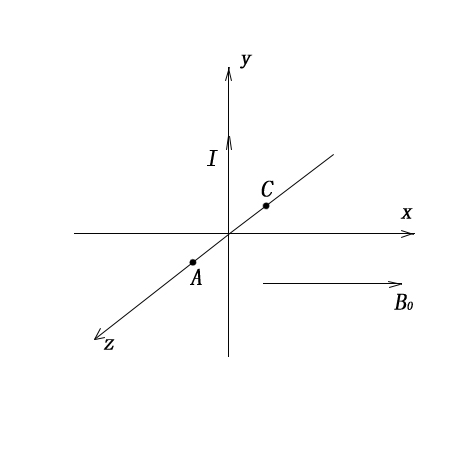
\includegraphics[width=15em, height=15em]{Chp8_illus1.jpg}
	\caption{练习5示意图}
	\label{fig:c8-t5}
\end{figure}

\solve
如图\ref{fig:c8-t5},电流$I$在$AC$两点产生的磁感应强度为$B_1=\frac{\mu_0I}{2\pi\cdot2}=10^{-6}T$,在$A$处方向为$x$轴正向,在$C$处方向为$x$轴负向;所以,$A$点处$B_0$与$B_1$叠加后的$B_A=2\times10^{-6}T$,$C$点处$B_0$与$B_1$叠加后的$B_C=0$.

\exercise{6}B

\solve
磁矩$\mu=i\cdot S$,边长扩大3倍,面积扩大9倍,磁矩扩大9倍.

\exercise{7}A

\begin{figure}[htbp]  % 可以使用figure来导入图片
	\centering
	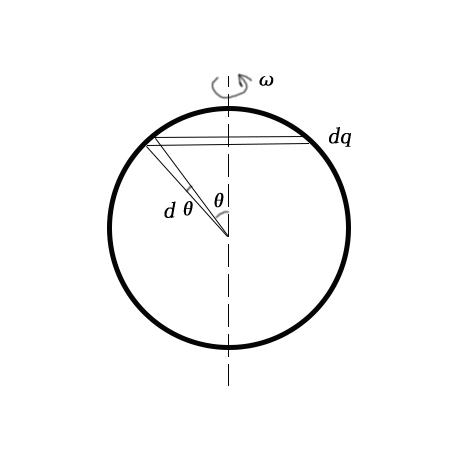
\includegraphics[width=15em, height=15em]{Chp8_illus2.jpg}
	\caption{练习7示意图}\label{fig:c8-t7}
\end{figure}

\solve
如图\ref{fig:c8-t7}所示,取$\di\theta$的微元,所以$\di q=2\lambda R\di\theta$,所以电流微元$\di I=\frac{\di q}{t}=\frac{2\lambda R\di\theta}{\frac{2\pi}{\omega}}=\frac{\lambda\omega R\di\theta}{\pi}$,磁矩微元$\di\mu=\di I\cdot S=\frac{\lambda\omega R\di\theta}{\pi}\cdot\pi(R\sin\theta)^2=\lambda\omega R^3\int_0^\pi\sin^2\theta\di\theta=\frac{\pi\lambda\omega R^3}{2}$.

\exercise{8}B

\solve
根据安培环路定理可得$B\cdot 2\pi r=\mu_0I$,代入数据计算出$I=1.4$A.

\exercise{9}B

\solve
环路$L$所围的电流$\sum I=0$,所以$\oint_L\vec{B}\cdot\di\vec{l}=0$,但环路$L$上每一点的磁感应强度$B$均垂直于环路$L$,故任一点$B\ne0$.

\exercise{10}C

\solve
竖直摆放的导线1在$M$、$N$点处产生的磁感应强度方向垂直纸面向里,记为$B_1$,水平摆放的导线2在$M$处产生的磁感应强度垂直纸面向里,在$N$处产生的磁感应强度垂直纸面向外,大小记为$B_2$;故$B_M=B_1+B_2$,$B_N=B_1-B_2$,即有$B_M>B_N$.

\section{填空题}
\exercise{11} 0

\analysis
根据空间位置关系,线圈$abcd$绕$cd$边旋转60°角后,恰好全部离开磁场,所以磁通为0.

\exercise{12} 0

\analysis
由对称性,$ab$间的每一条导线上的电流均为$\frac{I}{4}$,每一个半圆环在环中心处产生的磁感应强度恰好与与之相对的半圆环在环中心处产生的磁感应强度大小相等,方向相反,四个圆环相叠加后环中心处总的磁感应强度为0.

\exercise{13} 1:1

\solve
由无限长直导线的磁感应强度公式可知,$B=\frac{\mu_0I}{2\pi r}$.所以,设$S_1$和$S_2$的宽度均为$l$,$\Phi_1=\int_a^{2a}B(r)l\di r=\frac{\mu_0Il}{2\pi}\ln2$,$\Phi_2=\int_{2a}^{4a}B(r)l\di r=\frac{\mu_0Il}{2\pi}\ln2$,比值为1:1.

\exercise{14} $\frac{\mu_0I}{4R}\vec{i}+\frac{\mu_0I}{2\pi R}\vec{k}$

\solve
$yOz$平面上的半圆环在$O$点产生的磁感应强度为$\vec{B_1}=\frac{\mu_0I}{4R}\vec{i}$,两条半长直导线在$O$点处产生的磁感应强度为$\vec{B_2}=2\cdot\frac{\mu_0I}{4\pi R}\vec{k}$,所以总磁感应强度为$B=\frac{\mu_0I}{4R}\vec{i}+\frac{\mu_0I}{2\pi R}\vec{k}$


\exercise{15} 1

\analysis
无限长载流螺线管内的磁感应强度大小为$B=\mu_0nI$,式中,$n$为单位长度上的匝数,$I$为通过导线的电流,故无限长载流螺线管在管内的磁感应强度与螺线管的半径无关,所以$\frac{B_R}{B_r}=1$.

\exercise{16} $\frac{\mu_0ih}{4\pi^2R^2}$

\solve
首先在狭缝处补上一个宽度为$h$,电流为$I=\frac{h}{2\pi R}i$的电流,则将原无限长导体薄管凑成了一整个无限长导体薄管,根据对称性,这个无狭缝的无限长导体薄管在其轴线上产生的磁感应强度为0;再在原狭缝处补上一个宽度为$h$,电流为$I=-\frac{h}{2\pi R}i$的电流,这一电流在管轴线上产生的磁感应强度大小为$B=\frac{\mu_0ih}{4\pi^2R^2}$即为管轴线处实际的磁感应强度大小.

\exercise{17} $4\pi\times10^{-6}$


\solve
密绕细长直螺线管在管内产生的磁场为匀强磁场,其磁感应强度为$B=\mu_0nI=4\pi\times10^{-7}\cdot\frac{10}{0.01}\cdot10=4\pi\times10^{-3}T$,磁通为$\Phi=BS=4\pi\times10^-3\cdot10\time10^{-4}=4\pi\times10^{-6}Wb$.

\exercise{18} $\frac{\mu_0I}{4\pi R}$

\solve
长直导线1在$O$点处产生的磁感应强度为$0$;流过$ab$劣弧的电流为$\frac{3}{4}I$,流过$ab$优弧的电流为$\frac{1}{4}I$,再次根据对称性,可知$ab$劣弧和$ab$优弧在$O$点处产生的磁感应强度和为0;最后只剩下长直导线2,它在$O$点处产生的磁感应强度$B=\frac{\mu_0I}{4\pi R}$即为$O$点处的磁感应强度大小.

\exercise{19} $\frac{\sqrt{2}\mu_0I\di l}{16\pi}$\quad $z$轴正向

\solve
电流元$I\di\vec{l}$距离$P$点的距离为$\sqrt{2}$,由毕奥萨法尔定律,$P$点处
\begin{equation*}
\di B=\frac{\mu_0}{4\pi}\cdot\frac{I\di l\cdot\sin\frac{3\pi}{4}}{2}=\frac{\sqrt{2}\mu_0I\di l}{16\pi}
\end{equation*}

\exercise{20} 0\quad$-\mu_0 I$

\analysis
$A$与$B$在$P$点产生的磁感应强度大小相等,方向相反,故$B_p=0$.如题图所示环路方向,结合安培环路定理可知$\oint_L\vec{B}\cdot\di\vec{l}=-\mu_0 I$.

\section{计算题}
\exercise{21}

\solve
在圆盘上取半径从$r$到$r+\di r$的一个圆环微元.

这个圆环微元产生的等效电流大小为
\begin{equation*}
i=\frac{q}{t}=\frac{2\pi r\di r\cdot\sigma}{\frac{2\pi}{\omega}}=\sigma\omega r\di r
\end{equation*}
所以,这个圆环微元在盘心产生的磁感应强度为
\begin{equation*}
\di B=\frac{\mu_0}{4\pi}\cdot\frac{i\cdot2\pi r}{r^2}=\frac{\mu_0i}{2r}=\frac{1}{2}\mu_0\sigma\omega\di r
\end{equation*}
所以
\begin{equation*}
B=\int_0^R\di B=\int_0^R\frac{1}{2}\mu_0\sigma\omega\di r=\frac{1}{2}\mu_0\sigma\omega R
\end{equation*}
方向与$\vec{\omega}$相同.

\exercise{22}

\solve 
由对称性,平面$y=0$上$B=0$,且磁场在$\vec{k}$方向上的分量大小为$0$.

取一个与$xOy$面平行的环路,其一边在$y=0$的平面上,另一边在$y=y$的平面上,宽为$l$.

由安培环路定理,当$|y|\le d$时,有
\begin{equation*}
B(y)\cdot l=\mu_0\sigma ly
\end{equation*}
当$|y|>d$时,有
\begin{equation*}
B(y)\cdot l=\mu_0\sigma ld
\end{equation*}
所以
\begin{equation*}
B(y)=
\begin{cases}
\mu_0\sigma|y|\qquad|y|\le d\\
\mu_0\sigma d\qquad|y|>d
\end{cases}
\end{equation*}
当$y>0$时,方向沿$x$轴负向;当$y<0$时,方向沿$x$轴正向.

\exercise{23}

\solve
对于半径为$R$的大圆环来说,记在距其环心距离为$x$处的磁感应强度为$B(x)$
\begin{equation*}
B=\frac{\mu_0IR^2}{2(R^2+x^2)^{\frac{3}{2}}}
\end{equation*}
由题目假设$x\gg R$,所以$B(x)=\frac{\mu_0IR^2}{2x^3}$。又有$x\gg R\gg r$,所以可近似视半径为$r$的圆环处磁感应强度为一常数.综上,小线圈中的磁通量为
\begin{equation*}
\Phi=B\cdot S=\frac{\mu_0IR^2}{2x^3}\cdot \pi r^2=\frac{\pi\mu_0Ir^2}{2k^3R}
\end{equation*}

\exercise{24}

\solve
在$O'$处填补与$I$方向、密度均相同的电流$I_1$和与$I$方向相反、密度相同的电流$I_2$
\begin{equation*}
I_1=I_2=\frac{I}{\pi (R_1^2-R_2^2)}\cdot\pi R_2^2=\frac{R_2^2}{R_1^2-R_2^2}I
\end{equation*}

(1)由对称性,圆柱体$O$与填补上的$I_1$在圆柱体轴线上产生的$B=0$.只需考虑在$O'$处填补的电流$I_2$电流。由安培环路定理$B_1\cdot2\pi b=\mu_0I_2$,所以
\begin{equation*}
B_1=\frac{\mu_0I}{2\pi b}\cdot\frac{R_2^2}{R_1^2-R_2^2}
\end{equation*}

(2)$I_2$在$O'$处轴线上产生的$B=0$,则只需考虑在$O$处的大圆柱电流产生的磁场即可。由安培环路定理$B_2\cdot2\pi b=\mu_0\frac{I}{R_1^2-R_2^2}b^2$,所以
\begin{equation*}
B_2=\frac{\mu_0I}{2\pi}\cdot\frac{b}{R_1^2-R_2^2}
\end{equation*}

\chapter{恒定磁场(二)}%第九章
\section{选择题}

\exercise{1}A

\solve 
见课本。

\exercise{2}C

\solve 
见课本。

\exercise{3}B

\solve
质谱仪原理。由左手定则或带电粒子受洛伦兹力矢量式知偏转方向向上。注意粒子y坐标变化量为二倍半径。

\exercise{4}B

\solve
由左手定则易判断电荷正负。由$v=\dfrac{qBr}{m}$知,半径越大,速率越大。

\exercise{5}A

\solve
设磁化电流强度$I_\text{磁}$。
由安培环路定理:
\begin{gather*}
H\cdot 2\pi R=I\\
B\cdot 2\pi R=\mu_0(I-I_\text{磁})
\end{gather*}
而
\[
H=\dfrac{B}{\mu_0\mu_r}
\]
联立得:
\[
I_\text{磁}=(1-\mu_r)I
\]
故
$\sigma_\text{磁}=\dfrac{I_\text{磁}}{2\pi R}=\dfrac{(1-\mu_r)I}{2\pi R}$
\footnotemark[1]
\footnotetext[1]{注意,磁化电流面密度的量纲是A/m而非$\textrm{A/m}^2$。}

\exercise{6}D

\solve
见课本。所谓“真空中相对磁导率”为1。

\exercise{7}D

\solve
磁感应强度对应$y$轴,饱和磁感应强度显然为线段OI。

\exercise{8}A

\solve
磁化率定义为$\mu_r-1$。磁化率大于$0$但很小的即为顺磁性物质。

\exercise{9}B

\solve
这是一个基本的模型。可以参考课本(黑皮)上册\rm{P}373例9.6。

取距离圆心为$r$、宽度为$\di{r}$的圆环为面积微元,各微元受力矩方向相同,则
\begin{gather*}
\di{I}=\dfrac{\omega}{2\pi}\sigma\cdot 2\pi r\di{r}=\omega\sigma r\di{r}\\
\|\di{\textbf{m}}\|=\di{I}\cdot \pi r^2=\pi\omega\sigma r^3\di{r}\\
\|\textbf{M}\|=\int_{0}^{R}\|\di{\textbf{m}}\times \textbf{B}\|=\int_{0}^{R}B\pi\omega\sigma r^3\di{r}=\dfrac{\pi\sigma\omega BR^4}{4}
\end{gather*}

\exercise{10}A

\solve
由$M=m\times B$
\footnotemark[2]
\footnotetext[2]{课本中只说明了该式对任何形状的闭合线圈成立。如果磁铁的尺寸远小于磁场的尺度,那么可将磁铁看作磁偶极子,该式亦成立,且$m$的方向为南极指向北极。}
可得答案。

\section{填空题}

\exercise{11}$\dfrac{a}{3}$

\solve
由$B=\dfrac{\mu_0I}{2\pi r}$,$AB$受两导线的磁场的安培力等大反向,故$\dfrac{1}{x}=\dfrac{2}{a-x}$,解得$x=\dfrac{a}{3}$。

\exercise{12}$9.33\times 10^{-19}$A/$\rm{m}^2$ \quad 相反

\solve
\begin{align*}
m&=IS\\
&=\dfrac{e}{T}\cdot \pi r^2\\
&=\dfrac{e^2B}{2\pi m}\cdot \pi\dfrac{m^2v^2}{e^2B^2}\\
&=\dfrac{mv^2}{2B}
\end{align*}
代入数据($m=9.1\times 10^{-31}$kg)即得结果。
\begin{figure}[!h]	
	\centering	
	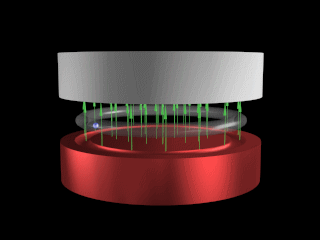
\includegraphics[width=0.5\textwidth]{Chp9_illus1.png}	
	\caption{练习12 示意图}\label{fig:c9-t12}
\end{figure}
如图\ref{fig:c9-t12},电子逆时针运动(俯视),其磁矩方向向下,故填“相反”。

\exercise{13}$BIR$\quad 垂直于纸面向里

\solve
$F=\int \|I\di{l}\times B\|$。在这里可以将该电流投影到垂直于$B$的方向上,等效为从a指向圆心的电流。投影长度为$R$,故安培力大小为$BIR$,方向用等效的电流判断即可。

\exercise{14}$0.226\textrm{T}$\quad 300\ \textrm{A/m}

\solve
“细环”指细螺绕环,内部磁感应强度可看做处处相等。由安培环路定理:
\begin{gather*}
H\cdot C=nI\\
H=\dfrac{nI}{C}=300\ \textrm{A/m}
\end{gather*}
即先算出第二空。那么
\[
B=\mu_0\mu_rH=72\pi\times 10^{-3}\textrm{T}=0.226\textrm{T}
\]

\exercise{15}$5.36\times 10^{-3}\textrm{kg}\cdot \textrm{m}^2/\textrm{s}^2$

\solve
由题,沿$y$轴方向的导线固定,故它以及垂直于$y$轴的导线受的力矩均不影响线圈的运动。设边长为$a$,转动轴在$y$轴上,剩下一根导线受的力沿$x$轴负方向,则力矩为
\begin{align*}
M&=Fa\sin\ang{40}\\
&=BIa^2\sin\ang{40}\\
&=7.2\sin\ang{40}\times 10^{-3}=5.36\times 10^{-3}
\end{align*}
保持位置不变,需要一等大反向的力矩。

\exercise{16}$2.3\times 10^{-5}$\quad 顺

\solve
参见练习8。

\exercise{17}0.5T\quad $y$轴正方向

\solve
由受力情况2得,磁场沿$y$轴,与情况1中“$z$轴正方向”垂直,故$M=m\times B=mB$,$B=
\dfrac{M}{m}=0.5\textrm{T}$。

由情况1及$M=m\times B$也易判断$B$的方向。

\exercise{18}逆时针方向

\solve
若无安培力,圆柱体在重力作用下有沿斜面向下滚动的趋势,所以其力矩方向为垂直于纸面向里。
为使安培力力矩垂直于纸面向外,可知磁矩方向是垂直于斜面向上的,于是可判断电流方向。

或者使用安培力的左手定则亦可:需要使左侧的电流受力向左而右侧的向右,使圆柱体有上滚的趋势。

\exercise{19}0.402A

\solve
可以参考课本(黑皮)上册\rm{P}422例9.19。
\begin{figure}[!h]	
	\centering	
	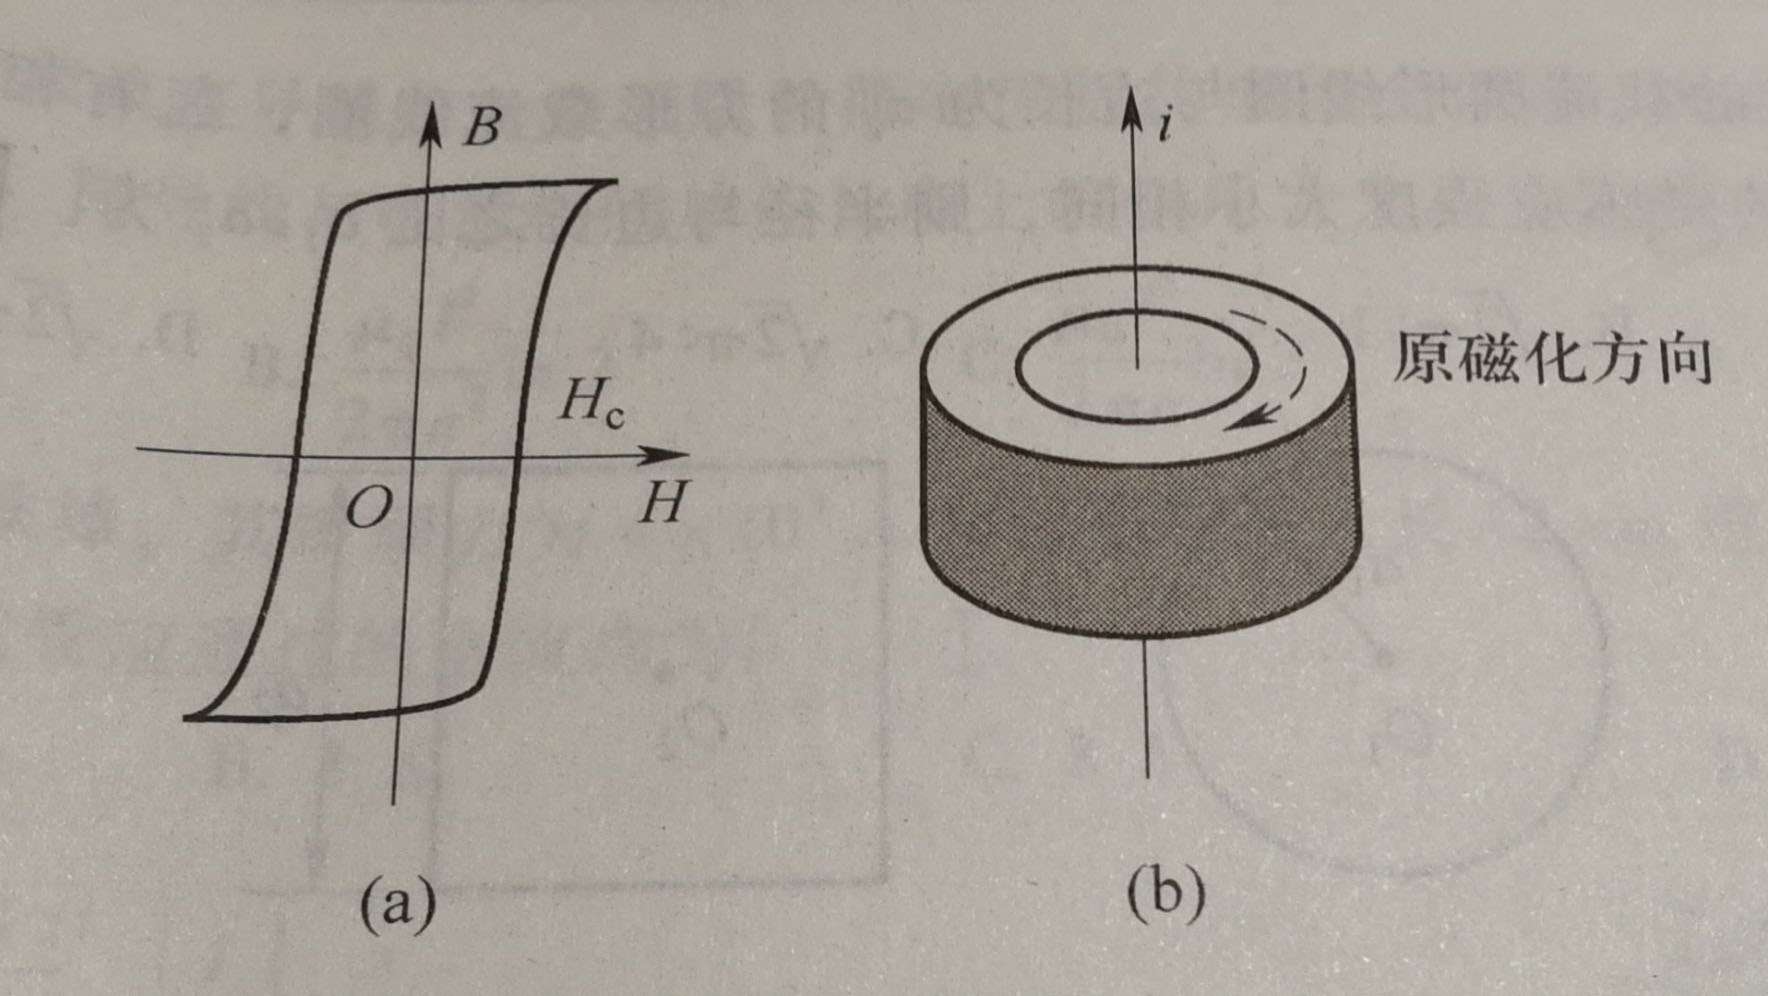
\includegraphics[width=0.5\textwidth]{Chp9_illus2.jpg}	
	\caption{练习19 示意图}
\end{figure}

根据其磁滞回线,磁化后的磁芯处于曲线与$B$轴交点处。由题意,外加磁场强度大小等于矫顽力。而由安培环路定理,$H=\dfrac{i}{2\pi r}$,半径越大,磁场强度越小。要使磁芯的磁化方向完全翻转,需要有:
\begin{gather*}
H_{R_2max}=\dfrac{i_{max}}{2\pi R_2}\geqslant H_c\\
i_{max}\geqslant 2\pi R_2H_c=2\pi\cdot \dfrac{0.8\textrm{mm}}{2} \cdot 160\textrm{A/m}=0.402\textrm{A}
\end{gather*}
注意题中给的是直径。

\exercise{20}居里点(居里温度)

\solve
见课本铁磁质部分。

\section{解答题}

\exercise{21}

\solve
由题,板间磁场水平向右,可取如题图所示的回路,其上方的水平部分(标箭头的部分)位于板间的任意位置,且只有在这段回路上磁场环量不为零。由安培环路定理,$Hl=\sigma l$,则
$H=\sigma=1000 \textrm{A/m}\footnotemark[3]$
\footnotetext[3]
{可以作为结论来记忆。真空中平行板电容器的电场亦有$D=\sigma$(电荷面密度)}

由$B,H,M$三者的关系得:
\begin{align*}
B&=\mu_0\mu_rH\\
&=4\pi\times 10^{-7}\times 500\times 1000 \textrm{T}\\
&=\dfrac{\pi}{5} \textrm{T}\\	
M&=\dfrac{B}{\mu_0}-H\\
&=(\mu_r-1)H\\
&=4.99\times 10^5 \textrm{A/m}
\end{align*}

\exercise{22}

\solve
由于各段导线为直线,写出其矢量式,利用安培力公式即可\footnotemark[4]。
\footnotetext[4]{题中已建系或自己建系时,可以用$\vec{i},\vec{j},\vec{k}$表示方向,也可以再用“$x$轴正向”等描述。}
\begin{gather*}
\vec{B}=0.6\vec{i}(\textrm{T})\\
F_{ab}=I\cdot 0.6\vec{j}\times 0.6\vec{i}=-1.44\vec{k}(N)\\
F_{bc}=I\cdot (0.6\vec{i}-0.6\vec{k})\times 0.6\vec{i}=-1.44\vec{j}(N)\\
F_{cd}=I\cdot (0.6\vec{k}-0.6\vec{j})\times 0.6\vec{i}=1.44(\vec{j}+\vec{k})(N)\\
F_{de}=I\cdot (-0.6\vec{k})\times 0.6\vec{i}=-1.44\vec{j}(N)\\
F_{ef}=I\cdot (-0.6\vec{i})\times 0.6\vec{i}=0
\end{gather*}

\exercise{23}

\solve
(1)由安培环路定理,可知距$AB$为$r$处的磁感应强度$B=\dfrac{\mu_0I_1}{2\pi r}$

以D为原点,$DN$、$DC$为$x$、$z$轴建立空间直角坐标系。

对CD:
\begin{gather*}
\vec{B}=\dfrac{\mu_0I_1}{2\pi d}\vec{j}\\
F_{CD}=I_2\cdot b\vec{k}\times \vec{B}=-\dfrac{\mu_0I_1I_2b}{2\pi d}\vec{i}
\end{gather*}

对MN:
\begin{gather*}
\vec{B}=\dfrac{\mu_0I_1}{2\pi (d+a)}\vec{j}\\
F_{MN}=I_2\cdot b(-\vec{k})\times \vec{B}=\dfrac{\mu_0I_1I_2b}{2\pi (d+a)}\vec{i}
\end{gather*}

对CM:
\[
\vec{B}=\dfrac{\mu_0I_1}{2\pi (d+x)}\vec{j}
\]
\begin{align*}
F_{CM}&=\int_{0}^{a}I_2\di{x}\cdot\vec{i}\times \vec{B}\\
&=\dfrac{\mu_0I_1I_2}{2\pi}\vec{k}\int_{0}^{a}\dfrac{\di{x}}{x+d}\\
&=\dfrac{\mu_0I_1I_2}{2\pi}\ln\dfrac{a+d}{d}\vec{k}
\end{align*}

对DN:
\[
\vec{B}=\dfrac{\mu_0I_1}{2\pi (d+x)}\vec{j}
\]
\begin{align*}
F_{DN}&=\int_{0}^{a}I_2\di{x}\cdot(-\vec{i})\times \vec{B}\\
&=-\dfrac{\mu_0I_1I_2}{2\pi}\vec{k}\int_{0}^{a}\dfrac{\di{x}}{x+d}\\
&=-\dfrac{\mu_0I_1I_2}{2\pi}\ln\dfrac{a+d}{d}\vec{k}
\end{align*}
(2)
\begin{align*}
F_\text{合}&=F_{CD}+F_{MN}+F_{CM}+F_{DN}\\
&=\dfrac{\mu_0I_1I_2b}{2\pi}(\dfrac{1}{d+a}-\dfrac{1}{d})\vec{i}\\
&=-\dfrac{\mu_0I_1I_2b}{2\pi d(d+a)}\vec{i}
\end{align*}

而$\vec{m},\vec{B}$均沿$y$轴正向,故$M=m\times B=0$
\footnotemark[5]。
\footnotetext[5]{对边受力不仅平行而且共线,线圈无转动趋势,所以力矩为零,不用考虑力矩是对哪个轴或点。}

\exercise{24}

\solve
电流密度$i=\dfrac{I}{\pi R^2-\pi r^2}$。
该系统可看作半径为$R$、电流密度为$i$的无限长圆柱面与半径为$r$、电流密度为$-i$的无限长圆柱面的组合。由安培环路定理和磁感应强度叠加原理(向下为正向):
\begin{gather*}
B_1\cdot 2\pi\cdot 2R=\mu_0i\cdot\pi R^2\\
B_2\cdot 2\pi\cdot (2R+d)=-\mu_0i\cdot\pi r^2\\
B_Q=B_1+B_2=\dfrac{\mu_0iR}{4}-\dfrac{\mu_0ir^2}{2(2R+d)}=\dfrac{\mu_0i}{2}(\dfrac{R}{2}-\dfrac{r^2}{2R+d})
\end{gather*}

\end{document}